\documentclass[sn-mathphys,Numbered]{sn-jnl}% Math and Physical Sciences Reference Style
%\documentclass[sn-mathphys,Numbered,draft]{sn-jnl}% Math and Physical Sciences Reference Style

%%\documentclass[sn-nature]{sn-jnl}% Style for submissions to Nature Portfolio journals
%%\documentclass[sn-basic]{sn-jnl}% Basic Springer Nature Reference Style/Chemistry Reference Style
%%\documentclass[sn-aps]{sn-jnl}% American Physical Society (APS) Reference Style
%%\documentclass[sn-vancouver,Numbered]{sn-jnl}% Vancouver Reference Style
%%\documentclass[sn-apa]{sn-jnl}% APA Reference Style 
%%\documentclass[sn-chicago]{sn-jnl}% Chicago-based Humanities Reference Style
%%\documentclass[default]{sn-jnl}% Default
%%\documentclass[default,iicol]{sn-jnl}% Default with double column layout

%%%% Standard Packages
%%<additional latex packages, if required can be included here>

\setlength{\parskip}{\baselineskip}

\usepackage{graphicx}%
\usepackage{amsmath,amssymb,amsfonts,bm}%
\usepackage{multirow}
\usepackage{amsthm}%
%\usepackage{subcaption}
\usepackage{mathrsfs}%
\usepackage[title]{appendix}%
\usepackage{xcolor}%
\usepackage{textcomp}%
\usepackage{manyfoot}%
\usepackage{booktabs}%
%\usepackage{algorithm}%
%\usepackage{algorithmicx}%
\usepackage{algpseudocode}%
\usepackage{listings}%
\usepackage{bigints}
\usepackage{outlines}
\usepackage{geometry}
\usepackage{subfigure}
\usepackage{siunitx}
\usepackage{float}
\usepackage{comment}

\geometry
{
a4paper,         % or letterpaper
textwidth=15cm,  % llncs has 12.2cm
textheight=24cm, % llncs has 19.3cm
% heightrounded,   % integer number of lines
% hratio=1:1,      % horizontally centered
% vratio=2:3,      % not vertically centered
}
\setlength{\tabcolsep}{0.5cm}
\usepackage[onehalfspacing]{setspace}
% \usepackage{lineno}
% \linenumbers
%%%%

\usepackage[utf8]{inputenc}
\usepackage{graphicx}
\usepackage[ruled,vlined]{algorithm2e}
\usepackage{amsmath}
%\usepackage{movie15} %to allow movie embedding
\usepackage[section]{placeins}
\usepackage{enumitem}
\usepackage{color,soul}
\usepackage{xfrac}

%% New math commands
\newcommand{\s}[1]{\overset{*}{#1}}
\newcommand{\RM}{\bm{\Lambda}}
\newcommand{\RMI}{\bm{\Lambda}_0}
\newcommand{\RMT}{\bm{\Lambda}_t}
\newcommand{\RV}{\bm{\psi}}
\newcommand{\magRV}{\psi}
\newcommand{\RMTS}{\s{\bm{\Lambda}}_t}
\newcommand{\bb}{\boldsymbol}
\usepackage{nicefrac}
%\usepackage{tikz}
%\usepackage{tikz-3dplot}
\usepackage{mathtools}

%% For contact
\newcommand{\rbar}{\bar{\bm{r}}}
\newcommand{\xibar}{\bar{\xi}}
%\newcommand{\magRV}{\bbit{\psi}}
\newcommand{\diag}{\rm diag}

%% Author notes for drafting (remove before submission).
%% \todo{...}     conspicuous block note; breaks across pages
%% \citetodo{...} placeholder for a citation not yet in bibliography.bib
\newcommand{\todo}[1]{\par\noindent\textcolor{red}{\rule{\linewidth}{0.8pt}}\par\nopagebreak
	\noindent{\small\color{red!70!black}\textbf{AUTHOR NOTE:} #1\par}\nopagebreak
	\noindent\textcolor{red}{\rule{\linewidth}{0.8pt}}\par}
\newcommand{\citetodo}[1]{\textcolor{red}{[\textbf{cite:}~#1]}}

\begin{document}

\title[Article Title]{A quasi-monolithic cell-centred finite volume approach for fluid-solid interaction}

\author*[1]{\fnm{Philip} \sur{Cardiff}}\email{philip.cardiff@ucd.ie}
%\author*[1,2,3]{\fnm{Philip} \sur{Cardiff}}\email{philip.cardiff@ucd.ie}
%\author[1,2,3]{\fnm{Dylan} \sur{Armfield}}
%%\author[5]{\fnm{Hiroaki} \sur{Nishikawa}}
%\author[4]{\fnm{\v{Z}eljko} \sur{Tukovi\'{c}}}
\author[1,2]{\fnm{Ivan} \sur{Batisti\'{c}}}
\author[1]{Add others}

\affil[1]{\orgdiv{School of Mechanical and Materials Engineering}, \orgname{University College Dublin}, \orgaddress{\country{Ireland}}}
%\affil[2]{\orgdiv{UCD Centre for Mechanics}, \orgname{University College Dublin}, \orgaddress{\country{Ireland}}}
%\affil[3]{\orgdiv{I-Form Centre}, \orgname{University College Dublin}, \orgaddress{\country{Ireland}}}
\affil[2]{\orgdiv{Faculty of Mechanical Engineering and Naval Architecture}, \orgname{University of Zagreb}, \orgaddress{\country{Croatia}}}
%\affil[5]{\orgname{National Institute of Aerospace}, \orgaddress{\country{Hampton, VA 23666, USA}}}



\abstract{
Fluid--solid interaction (FSI) problems arising in engineering and biomedical applications often involve strong coupling and significant added-mass effects, regimes in which partitioned solution strategies can suffer from slow convergence or instability.
Monolithic solution strategies provide an attractive alternative but have been developed almost exclusively in the finite element setting.
This paper presents a quasi-monolithic cell-centred finite volume method for FSI, in which the fluid velocity and pressure (in arbitrary Lagrangian--Eulerian form) and solid velocity (in total Lagrangian form) momentum equations are coupled within a single nonlinear residual, with strong enforcement of the interface kinematic and dynamic conditions.
The coupled nonlinear system is solved using a Jacobian-free Newton--Krylov procedure with an approximate block preconditioner, assembled from compact finite volume linearisations of the fluid, solid, and interface-coupling terms.
The preconditioner supports both monolithic and nested field-split usage, with optional Schur-complement approximation of the velocity--pressure block via the Rhie--Chow pressure stabilisation.
The method is implemented in the OpenFOAM-based toolbox solids4foam using PETSc for the nonlinear and linear algebra.
Performance is assessed on a suite of established two- and three-dimensional FSI benchmarks, demonstrating second-order spatial and temporal accuracy, agreement with partitioned reference solutions, and robust convergence at time-step sizes for which partitioned coupling becomes inefficient or fails.
}

\keywords{Fluid--solid interaction, Monolithic, Quasi-monolithic, Jacobian-free Newton--Krylov, Finite volume method, Added-mass effects, solids4foam, OpenFOAM}

\maketitle

\todo{The title, abstract, Introduction (Section~\ref{sec:intro}) and Sections~\ref{sec:math_model}--\ref{sec:numerical_methods} are still those of the parent quasi-monolithic FSI paper and have deliberately not been rewritten in this pass. The verification evidence in Sections~\ref{sec:verification_methodology}--\ref{sec:recommended_suite} uses only the partitioned solution procedures (IQN-ILS, Robin--Neumann, Aitken); the quasi-monolithic solver is not used as evidence. Section~\ref{sec:numerical_methods} must eventually describe the partitioned procedures that produced the results.}


%%%%%%%%%%%%%%%%%%%%%%%%%%%%%%%%%%%%%%%%%%%%%%%%%%%%%%%%%%%%%%%%%%
%%%%%%%%%%%%%%%%%%%%%%%%%%%%%%%%%%%%%%%%%%%%%%%%%%%%%%%%%%%%%
\section{Introduction}\label{sec:intro}
%%%%%%%%%%%%%%%%%%%%%%%%%%%%%%%%%%%%%%%%%%%%%%%%%%%%%%%%%%%%%
Benchmark problems are central to the development of fluid--solid interaction (FSI) codes: they are used to demonstrate accuracy, to compare coupling algorithms and to support claims that a new method is correct.
Many such problems exist, from the flag-behind-a-cylinder family of \citet{Turek2006} to pressure-pulse tubes, lid-driven cavities with flexible membranes and three-dimensional flows past elastic plates.
Far fewer of them come with a benchmark \emph{solution} whose own numerical error has been established: published values are often single-mesh results, are read from figures, are reported without time-step studies, or differ between sources by more than the discretisation errors that they are used to judge.
Agreement with such a value is then weak evidence, and disagreement is ambiguous: it may mean that the code under test is wrong, that the reference is wrong, or that the code's own solution is not yet resolved.
This paper addresses that gap for continuum FSI with an open, executable verification suite in which the quality of every reference and the spatial, temporal and iterative errors of every result are stated explicitly.

FSI methods can be classified along three axes: the modelling viewpoint (Eulerian, Lagrangian, or mixed), the degree of interface coupling (weak vs.\ strong), and the solver structure (partitioned vs.\ monolithic).

Eulerian approaches treat both solid and fluid domains as ``fluid-like'' (e.g.\ volume-of-fluid~\citep{jain2019conservative}, level-set~\citep{dunne2006eulerian, cottet2008eulerian}), easily allowing arbitrarily large solid deformations, but conservative interface descriptions and the inclusion of advanced solid constitutive laws remain challenging.
In contrast, Lagrangian (particle-type) approaches treat both domains as ``solid-like'', e.g.\ smooth-particle hydrodynamics, the material point method, and the particle finite element method (PFEM)~\citep{aubry2005particle, aubry2006fractional, cremonesi2020state}.
These methods are promising for large-deformation problems but typically come with a prohibitive computational cost.
Mixed Eulerian--Lagrangian approaches treat the solid (and interface) as Lagrangian and the fluid using an arbitrary Lagrangian--Eulerian (ALE) description.
ALE is effective for small to moderate interface deformations but eventually fails for very large deformations~\citep{wall2006large}, motivating methods that allow the solid to ``float over'' an Eulerian fluid grid, such as immersed boundary/domain~\citep{peskin1977numerical, peskin2002immersed, iaccarino2003immersed}, Chimera/overset~\citep{ge2003three, miller2014overset, li2021fluid, cane2021patient}, and cut-cell methods~\citep{pasquariello2016cut, tao2020new, xie2020cartesian}.
Of these, overset methods offer large-deformation freedom while retaining orthogonal interface cells suitable for resolving fluid boundary layers, albeit with the downside of greater implementation complexity.

In weakly coupled (loosely coupled) approaches, the fluid and solid are solved once per time step without iteration over the interface conditions~\citep{farhat2000two}.
This is computationally inexpensive but unstable for strongly coupled systems with significant added-mass effects~\citep{Causin2005, Forster2006}, such as incompressible flows interacting with light, flexible structures.
Strongly coupled approaches strictly enforce the interface kinematic and dynamic conditions at each time step; the present work focuses on the strongly coupled case.

Strong coupling can be enforced through either a partitioned or a monolithic solver structure.
In partitioned (staggered, two-system) approaches, separate solvers --- and potentially separate discretisations --- are used for the fluid and solid~\citep{Tukovic2018}, and outer iterations are performed over the interface at each time step.
These are accelerated using Aitken relaxation~\citep{Degroote2009, bungartz2016precice, irons1969version, kuttler2008fixed}, quasi-Newton schemes~\citep{santiago2020hpc, delaisse2022surrogate}, or Robin-type interface conditions~\citep{Tukovic2018b}.
The principal limitations are robustness and efficiency: for strongly coupled, highly nonlinear problems, outer-iteration convergence can be slow or fail entirely, particularly under strong added-mass loading.
In contrast, monolithic approaches treat the fluid and solid as a single system, solved concurrently within the same linearised system~\citep{Degroote2009}.
This avoids outer iterations and can handle tightly coupled nonlinear problems robustly, at the cost of reduced modularity and a poorly conditioned linear system that is more difficult to solve.

The verification literature for FSI is smaller than that for its component fields.
The proposal of \citet{Turek2006} defines the most widely used problems and reports multi-level reference values, and goal-oriented error estimation has been developed for FSI in the finite element setting~\citep{Richter2012, Richter2017}; monolithic finite element and hybrid finite volume/finite element codes have been demonstrated on these and related problems~\citep{Heil2004, Heil2008, Eken2016, Lozovskiy2019}, with convergence evidence that ranges from multi-level studies to single-mesh results.
Partitioned finite volume FSI, including the OpenFOAM-based framework of \citet{Tukovic2018} on which the solids4foam toolbox~\citep{Cardiff2025} builds, has mostly been assessed by comparison with such published values.
Across this literature, the error of the reference itself is rarely quantified, iterative (coupling) errors are seldom separated from discretisation errors, and the time integration of a reference is often first order with a large step, so that two codes can disagree because their references differ rather than because either is wrong.
General verification practice --- observed orders from systematic refinement, separation of error sources, and the distinction between verification and validation~\citetodo{Roache 1998; Oberkampf \& Roy 2010} --- is well established for single-field problems but is applied unevenly to coupled FSI.

The present work applies that practice to a suite of continuum FSI benchmarks, all solved with one partitioned, cell-centred finite volume framework: a PIMPLE-type ALE fluid, small-strain and total Lagrangian finite volume solids with standard and high-order discretisations~\citep{Cardiff2026, Batistic2026}, and Dirichlet--Neumann (Aitken~\citep{kuttler2008fixed}, IQN-ILS~\citep{Degroote2009}) or Robin--Neumann~\citep{Tukovic2018b} coupling.
The aim is not to promote a solver but to establish, case by case, what the available references can and cannot verify, and how much of the remaining difference is attributable to the code under test.
Verification here means convergence of the discrete solution to the solution of the stated mathematical problem; agreement with experimental data is validation, is kept separate, and is never used as evidence of convergence.

The specific contributions are:
\begin{enumerate}
    \item A reference-quality classification for FSI benchmarks (category A: analytical; B: independently converged numerical solution, possibly of a problem with a small, quantified model-form difference; C: published values with incompletely quantified error; C-weak: digitised, single-mesh, inconsistent or same-lineage values), applied to every case in the suite.
    \item Spatial, temporal and iterative error studies for each benchmark, with observed orders reported only where the evidence supports them, and with the slowest-converging quantity of interest identified.
    \item Evidence that verification exposes real defects and misleading benchmark agreement: two solver defects found through a cross-platform discrepancy in a three-dimensional tube, one compiler-dependent and one that changed the interface interpolation with mesh level; a two-level agreement with the Hron--Turek FSI3 reference that disappears on a third level; a published code-to-code discrepancy that is largely reproduced by the difference in time integration; and a default coupling convergence test that can accept unconverged steps.
    \item An open, executable implementation of the suite in solids4foam~\citep{Cardiff2025}: case set-ups, verification drivers that compute the quantities of interest and observed orders, and machine-readable reference files with their provenance, so that the studies can be re-run on other codes and platforms.
\end{enumerate}

Section~\ref{sec:math_model} states the governing equations and Section~\ref{sec:numerical_methods} the partitioned finite volume procedures used for every result.
Section~\ref{sec:verification_methodology} sets out the verification methodology, Section~\ref{sec:benchmark_suite} presents the benchmark suite, Section~\ref{sec:cross_benchmark} draws cross-benchmark conclusions, and Section~\ref{sec:recommended_suite} proposes a recommended verification suite.
Section~\ref{sec:discussion} discusses the findings and Section~\ref{sec:conclusion} concludes.
\hl{Before submission, verify all references have correct details}

%%%%%%%%%%%%%%%%%%%%%%%%%%%%%%%%%%%%%%%%%%%%%%%%%%%%%%%%%%%%%%%%%%

%%%%%%%%%%%%%%%%%%%%%%%%%%%%%%%%%%%%%%%%%%%%%%%%%%%%%%%%%%%%%%%%%%
\input{sectionMathModel.tex}
%%%%%%%%%%%%%%%%%%%%%%%%%%%%%%%%%%%%%%%%%%%%%%%%%%%%%%%%%%%%%%%%%%


%%%%%%%%%%%%%%%%%%%%%%%%%%%%%%%%%%%%%%%%%%%%%%%%%%%%%%%%%%%%%%%%%%
%%%%%%%%%%%%%%%%%%%%%%%%%%%%%%%%%%%%%%%%%%%%%%%%%%%%%%%%%%%%%
\section{Numerical methods}\label{sec:numerical_methods}
%%%%%%%%%%%%%%%%%%%%%%%%%%%%%%%%%%%%%%%%%%%%%%%%%%%%%%%%%%%%%
% Every result in Sections 4-6 was produced with the partitioned procedures
% described here (solids4foam fluidSolidInterface: fixedRelaxation, Aitken,
% IQNILS; Robin condition elasticWallPressure). The experimental
% quasi-monolithic solver of the parent paper is not used; its description is
% preserved, outside the build, in sectionNumericalModelQuasiMonolithic.tex.
% Source checked: solids4foam development (src/solids4FoamModels:
% fluidModels/pimpleFluid, solidModels, fluidSolidInterfaces) and the case
% dictionaries of the tutorials in Section 5.

All results in this paper were obtained with the partitioned fluid--solid interaction framework of the open-source toolbox solids4foam~\citep{Cardiff2025}, which builds on the OpenFOAM finite volume library~\citep{Weller1998} and follows the partitioned approach of \citet{Tukovic2018}.
The fluid and the solid are discretised on separate cell-centred finite volume meshes and solved by separate field solvers, which exchange interface displacements and tractions within each time step.
This section summarises the components that determine the discretisation, temporal and iterative errors studied in Sections~\ref{sec:verification_methodology}--\ref{sec:cross_benchmark}; implementation detail is in the solids4foam source and in the case dictionaries that accompany each benchmark.
Case-specific choices (time scheme, convection scheme, solid variant, coupling algorithm and tolerances) are stated with each benchmark in Section~\ref{sec:benchmark_suite}.

%%--------------------------------------------------------------------------------------------------------------------%%
\subsection{Fluid}\label{sec:fluid_solver}
%%--------------------------------------------------------------------------------------------------------------------%%

The incompressible Navier--Stokes equations in ALE form (Section~\ref{sec:fluid_governing_eqn}) are solved by the \texttt{pimpleFluid} model, a solids4foam port of the OpenFOAM \texttt{pimpleFoam} solver.
Velocity and pressure are collocated at cell centres; the face fluxes are obtained by Rhie--Chow-type momentum interpolation~\citep{Rhie1983}, and the pressure--velocity coupling is the segregated PIMPLE algorithm (PISO pressure correctors within SIMPLE-type outer correctors), with the numbers of outer and pressure correctors stated per case.
Spatial operators are the standard second-order finite volume operators: midpoint quadrature, linear face interpolation, least-squares or Gauss cell gradients, and Laplacian face fluxes with explicit non-orthogonal correction~\citep{Jasak1996}.
Convection is discretised with central (\texttt{linear}) or limited linear-upwind interpolation, depending on the case.
The time derivative is discretised with the second-order backward difference formula (BDF2, \texttt{backward}) unless stated; implicit Euler is used only in the deliberate time-scheme comparison of Section~\ref{sec:3dtube}.
On the moving mesh the convective flux is the relative flux $\bb{\Gamma}_f\cdot(\bb{v}_f - \bb{v}^\Gamma_f)$, where the mesh flux $\bb{\Gamma}_f\cdot\bb{v}^\Gamma_f$ is the volume swept by face $f$.
With BDF2 the swept volumes of the last two steps are combined with the BDF2 weights, so that the discrete space-conservation law (Equation~\eqref{eqn:gcl}) holds for the backward volume derivative.
On the interface the fluid velocity equals the velocity of the moving wall, and the interface traction passed to the solid is the sum of the pressure and viscous tractions on the fluid interface faces.

\subsection{Fluid mesh motion}\label{sec:fluid_mesh_motion}

The interior fluid mesh follows the interface through a Laplacian equation for the cell motion velocity (\texttt{velocityLaplacian}), whose diffusivity varies with the inverse (in most cases the inverse square) of the distance to the moving boundaries, so that cells near the interface move almost rigidly~\citep{Tukovic2018}.
The interface displacement is the solid displacement transferred to the fluid interface (Section~\ref{sec:interface_transfer}); the point motion is obtained from the cell motion velocity by interpolation, and the mesh points are moved once per coupling iteration.
Mesh motion is a numerical device: it changes the discrete solution only through the mesh quality and through the space-conservation and moving-wall treatments described above.

%%--------------------------------------------------------------------------------------------------------------------%%
\subsection{Solid}\label{sec:solid_solver}
%%--------------------------------------------------------------------------------------------------------------------%%

The solid momentum equation (Section~\ref{sec:solid_model}) is discretised by a cell-centred finite volume method with the total displacement as unknown~\citep{Jasak2000, Cardiff2021}.
Two kinematic formulations are used: a small-strain (linear geometry) formulation for the linear-elastic walls (ringAddedMass, womersleyTube, 3dTube), and a total Lagrangian formulation for the finite-strain problems, with St Venant--Kirchhoff (Hron--Turek, collapsibleChannel, mokLidDrivenCavity) or neo-Hookean (Hessenthaler) material laws.
The time derivative uses BDF2, and each solid solve is a Newton--Krylov iteration through the PETSc SNES interface~\citep{PETSc, Cardiff2026}.
Two spatial variants are used.
The \emph{standard} variant uses a linear least-squares reconstruction of the displacement and a compact-stencil momentum stabilisation, a Rhie--Chow-type difference between the compact and the reconstructed face normal gradient, scaled by a user factor~\citep{Cardiff2026}; it is formally second order, but the stabilisation is not negligible on coarse meshes and stiffens thin, bending-dominated structures (Section~\ref{sec:fsi1}).
The \emph{high-order} variant evaluates the face fluxes of the residual from a cubic moving-least-squares reconstruction of the displacement~\citep{Batistic2026}.
Which variant is used is stated per case, because for thin bending-dominated walls the choice can dominate the coupled error (Section~\ref{sec:collapsible}).

%%--------------------------------------------------------------------------------------------------------------------%%
\subsection{Interface transfer}\label{sec:interface_transfer}
%%--------------------------------------------------------------------------------------------------------------------%%

Displacements are transferred from the solid to the fluid interface at the interface points, and tractions from the fluid to the solid interface at the faces.
Where the two interface meshes coincide (ringAddedMass, womersleyTube, collapsibleChannel, mokLidDrivenCavity), a direct one-to-one map is used.
Where they do not (Hron--Turek, 3dTube, Hessenthaler), face tractions are transferred conservatively with arbitrary-mesh-interface (AMI) weights, and point displacements by barycentric interpolation on a triangulation of the donor interface faces.
The interface transfer is part of the discretisation: it is an operator that must converge with refinement like any other, and in 3dTube a defect in it changed with mesh level (Section~\ref{sec:3dtube}).

%%--------------------------------------------------------------------------------------------------------------------%%
\subsection{Coupling algorithms}\label{sec:coupling_algorithms}
%%--------------------------------------------------------------------------------------------------------------------%%

Strong coupling is enforced by outer (coupling) iterations within each time step.
Two interface formulations are used.

\paragraph{Dirichlet--Neumann.}
The fluid receives the interface displacement (mesh motion and wall velocity) and the solid receives the fluid traction.
Each time step starts with a solid predictor, i.e.\ a solid solve with the fluid traction of the previous step, whose displacement is passed to the fluid without relaxation in the first iteration~\citep{Tukovic2018}.
Subsequent interface displacements are updated by fixed under-relaxation, by Aitken dynamic relaxation~\citep{kuttler2008fixed}, or by the interface quasi-Newton inverse least-squares method (IQN-ILS)~\citep{Degroote2009}, which builds an approximate inverse Jacobian of the interface residual from the secant information of the current and, optionally, previous time steps; secant columns that are repeated or nearly linearly dependent are filtered before the least-squares solve.

\paragraph{Robin--Neumann.}
The fluid pressure satisfies a Robin condition on the interface that accounts for the solid inertia through an estimate $\rho_S h_S$ of the solid interface impedance~\citep{Tukovic2018b}, and the iterations are unrelaxed fixed-point iterations.
The Robin condition modifies the discrete interface condition within the iterations; at convergence the interface flux is made consistent with the mesh motion.
Because it changes the iteration rather than only accelerating it, the converged Robin--Neumann and Dirichlet--Neumann solutions need not agree to the coupling tolerance (Section~\ref{sec:ref_hierarchy}).

\paragraph{Convergence test.}
The interface residual $\bb{r}$ is the difference between the solid interface point positions, transferred to the fluid interface, and the fluid interface point positions.
Two normalised measures are formed,
\begin{equation}
	r_1 = \frac{\|\bb{r}\|}{\max_k \|\bb{r}^{(k)}\|},
	\qquad
	r_2 = \frac{\|\bb{r}\|}{\|\bb{d}^\Gamma\|_{\max}},
	\label{eq:coupling_residuals}
\end{equation}
where the maximum in $r_1$ is over the coupling iterations $k$ of the current step and $\|\bb{d}^\Gamma\|_{\max}$ is the largest norm of the \emph{total} interface displacement seen so far.
In the legacy default a step is accepted when $\min(r_1, r_2)$ is below the coupling tolerance; a strict option requires $\max(r_1, r_2)$ to be below it.
The two tests differ greatly in slowly varying phases with a large total interface displacement, where $r_2$ can be small after a single relaxed iteration whatever the reduction of the residual within the step (Section~\ref{sec:iterative_errors}).
Robin--Neumann iterations additionally require the change of interface pressure and the interface leakage flux to fall below their own tolerances.
By default, a step that does not meet the test within the maximum number of iterations stops the run; the default test can nevertheless accept insufficiently converged steps, as shown in Section~\ref{sec:iterative_errors}.

%%--------------------------------------------------------------------------------------------------------------------%%
\subsection{Solution procedure and toolchain}\label{sec:implementation_details}
%%--------------------------------------------------------------------------------------------------------------------%%

The partitioned procedure for one time step is summarised in Algorithm~\ref{alg:partitioned_fsi}.

\begin{algorithm}[htbp]
\caption{Partitioned FSI procedure for one time step (solids4foam \texttt{fluidSolidInterface}).}
\label{alg:partitioned_fsi}
\begin{algorithmic}[1]
\State Advance time; solve the solid with the fluid traction of the previous step (predictor).
\State Transfer the predicted interface displacement to the fluid interface.
\State For coupling iterations $k = 1, 2, \ldots$, up to the maximum number:
\State \hspace{1.5em}move the fluid mesh to the current interface displacement and update the mesh fluxes;
\State \hspace{1.5em}solve the fluid (PIMPLE outer and pressure correctors) with the moving-wall velocity, or with the Robin pressure condition;
\State \hspace{1.5em}transfer the fluid interface traction to the solid and solve the solid (Newton--Krylov);
\State \hspace{1.5em}transfer the solid interface displacement to the fluid interface and evaluate $\bb{r}$, $r_1$ and $r_2$;
\State \hspace{1.5em}stop if the convergence test (and, for Robin--Neumann, the pressure and flux tests) is met;
\State \hspace{1.5em}otherwise update the interface displacement: fixed relaxation, Aitken, IQN-ILS, or none (Robin--Neumann).
\end{algorithmic}
\end{algorithm}

The calculations used the OpenCFD releases OpenFOAM-v2412 and OpenFOAM-v2512 with PETSc, on Linux (x86\_64) and, for some of the inexpensive cases, macOS; the release, platform and solids4foam commit are stated with each result.
The compiler and its optimisation level are recorded as part of the configuration: the default OpenFOAM build rules compile at \texttt{-O3}, whereas the EasyBuild toolchain used on one of the clusters compiles at \texttt{-O2}, and this difference exposed a solver defect (Section~\ref{sec:3dtube}).
\todo{State per case the exact solids4foam commit, OpenFOAM release, compiler and optimisation flags, PETSc version and platform (see Section~\ref{sec:qoi} and paper-data/manuscript\_update\_2026-10.md). Confirm that the predictor/relaxation description matches the commit used for each result (the \texttt{predictor} default changed in solids4foam PR \#492).}

%%%%%%%%%%%%%%%%%%%%%%%%%%%%%%%%%%%%%%%%%%%%%%%%%%%%%%%%%%%%%%%%%%


%%%%%%%%%%%%%%%%%%%%%%%%%%%%%%%%%%%%%%%%%%%%%%%%%%%%%%%%%%%%%%%%%%
% Sections 4--8: verification-benchmark paper.
% The parent (monolithic-solver) test-case section is preserved unchanged in
% sectionTestCases.tex but is no longer part of the build: its results come
% from the experimental quasi-monolithic solver, which is not used as
% verification evidence in this paper.
%%%%%%%%%%%%%%%%%%%%%%%%%%%%%%%%%%%%%%%%%%%%%%%%%%%%%%%%%%%%%%%%%%%
\section{Test Cases}\label{sec:test_cases}
%%%%%%%%%%%%%%%%%%%%%%%%%%%%%%%%%%%%%%%%%%%%%%%%%%%%%%%%%%%%%%%%%%
% Briefly state what is assessed in the test cases, and what each new test case adds.
%
% What do we want do demonstate? Some ideas (many of which can be merged)
%
% - accuracy => do we get the same answer as partitioned (in the limit of mesh/time-step refinement) => this is surely the first thing to check; we can dedicate the first case or cases to this, or simply include reference data and comparisons for all cases.
%
% - efficiency => execution time and RAM usage of monolithic vs partitioned
%
% - robustness => when might partitioned crash when monolithic does not => it seems that monolothic allows larger stable time steps compared with partitioned, which is important to highlight (e.g. cavity case seems to work with any time step, while partitioned needs small time step)
%
%
% - effect of preconditioner is important
%
% - scalability => iteration (Newton and Krylov behaviour) count, wall time, memory growth with case size and also parallel scaling
%
% - added mass sensitivity => this is where monolithic should shine; maybe a closed domain case
% - coupling strength => we could vary density, viscosity, flow speed to demonstrate this; this could be done with one case (with different parameters) or via multiple case (where the cases span a range of behaviours)
%
% - linear vs highly nonlinear case (in terms of solid behaviour), e.g large solid deformations, large fluid mesh motions
%
% - solution quality as a function of time step size for monlithic vs partitioned
%
The test cases are designed to assess the proposed monolithic solver from several complementary perspectives. First, \emph{accuracy} is examined by comparing against benchmark solutions and by checking mesh- and time-step-converged responses. Second, \emph{robustness} is assessed by considering strongly coupled problems for which partitioned procedures may require smaller stable time steps or may fail to converge. Third, \emph{efficiency} is evaluated in terms of wall-clock time, memory usage, and nonlinear/linear iteration counts. In addition, the suite is chosen to expose solver characteristics that are particularly relevant for a monolithic approach, including sensitivity to preconditioning, coupling strength and added-mass effects, scalability with problem size, and behaviour for both mildly and highly nonlinear structural and mesh deformations. Accordingly, each case adds a distinct challenge, spanning simple internal-flow verification problems, established FSI benchmarks, temporal-accuracy studies, and progressively more demanding two- and three-dimensional configurations.

\hl{Should we examine the fluid convection linearisation option (extrapolate flux)?}
\hl{If not, note this as a difference to the original Liu approach}

%%--------------------------------------------------------------------------------------------------------------------%%
\subsection{Case 1: Channel flow over a cavity with a flexible bottom} \label{sec:case1}
%%--------------------------------------------------------------------------------------------------------------------%%
Two-dimensional steady laminar flow in a channel over a cavity was proposed as a fluid dynamics benchmark in \citep{Juretic2010} and was later proposed as a fluid-solid interaction benchmark through addition of a flexible solid plate as a lower wall by \citet{Tukovic2018} (Figure \ref{fig:cavity_geom}).
The test is used here to assess robustness and convergence behaviour for an internal-flow fluid-solid interaction problem with a compliant wall.

\begin{figure}[htbp]
	\centering
	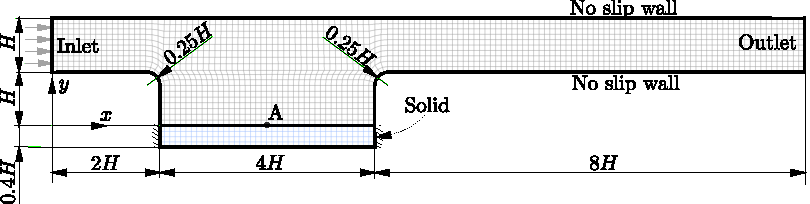
\includegraphics[scale=1]{figures/cavityFlexibleBottom-geometry}
	\caption{Case 1 setup (channel flow over a cavity with a flexible bottom), including geometry, boundary conditions, and representative mesh.}
	\label{fig:cavity_geom}
\end{figure}

The fluid domain has channel height $H = 1\,\mathrm{m}$ and is solved as incompressible, Newtonian, and isothermal, with density $\rho_f = 1\,\mathrm{kg/m^3}$ and kinematic viscosity $\nu_f = 0.01\,\mathrm{m^2/s}$. A parabolic inlet velocity profile with mean value $\bar{u}_{\mathrm{in}} = 1\,\mathrm{m/s}$ is imposed, corresponding to $Re = 100$ based on $H$. A fixed pressure of $0$ Pa is prescribed at the outlet, while no-slip conditions are applied on fluid walls and interface-consistent kinematic/dynamic coupling conditions are enforced at the fluid-solid boundary.
The flexible cavity bottom is modelled as a Saint Venant--Kirchhoff solid with density $\rho_s = 1000\,\mathrm{kg/m^3}$, Young's modulus $E = 500$ Pa, and Poisson's ratio $\nu_s = 0.4$.
To efficiently and robustly obtain the steady-state solution, the simulation is advanced in time until a steady response is reached, with a damping coefficient $c_d = 0.1$ s$^{-1}$ applied to the solid.
% \hl{check: I may scale this with time step size}.

\begin{table}[htbp]
	\centering
	\begin{tabular}{llll}
		\hline
		Quantity & Symbol & Value & Unit \\
		\hline
		Channel height & $H$ & 1 & m \\
		Mean inlet velocity & $\bar{u}_{\mathrm{in}}$ & 1 & m/s \\
		Fluid density & $\rho_f$ & 1 & kg/m$^3$ \\
		Fluid kinematic viscosity & $\nu_f$ & 0.01 & m$^2$/s \\
		Solid density & $\rho_s$ & 1000 & kg/m$^3$ \\
		Young's modulus & $E$ & 500 & N/m$^2$ \\
		Poisson's ratio & $\nu_s$ & 0.4 & -- \\
		\hline
	\end{tabular}
	\caption{Primary Case 1 parameters, following the \texttt{cavityFlexibleBottom} tutorial setup.}
	\label{tab:case1_parameters}
\end{table}

Following the approach in \citep{Tukovic2018}, the prediction of two quantities are assessed: (i) the displacement history of a monitoring point on the flexible plate (point $A=(4,-1,0)$) and (ii) the resultant force components acting on the fluid-solid interface. 
A systematic mesh- and pseudo-time-step sensitivity study was performed using three uniformly refined meshes and six pseudo-time-step sizes. The mesh spacings considered were
\[
    \Delta x \in \{0.1,\;0.05,\;0.025\}\,\mathrm{m},
\]
while the pseudo-time-step sizes were
\[
    \Delta t \in \{0.5,\;1,\;2.5,\;5,\;10,\;20\}\,\mathrm{s}.
\]
For each run, the computation was advanced until the automatic steady-state criterion was satisfied, based on the relative change in the monitored displacement and interface force over consecutive time levels. Cases that did not satisfy the steady-state criterion before the prescribed final time were excluded from the solution-sensitivity plots.

Figure~\ref{fig:cavity_solution_sensitivity} shows the dependence of the steady-state vertical displacement at point $A$ and the vertical resultant interface force on the mesh spacing and pseudo-time-step size. The results show a clear dependence on spatial resolution, with both $U_y$ and $F_y$ varying monotonically under mesh refinement. In contrast, for a fixed mesh, the variation with pseudo-time-step size is small over the range of values considered. This indicates that, once the computation has reached the steady-state criterion, the pseudo-time-step size has only a weak influence on the predicted steady response. The dominant numerical sensitivity for this case is therefore associated with spatial discretisation rather than pseudo-time advancement.

\begin{figure}[htbp]
    \centering

    \subfigure[Vertical displacement at point $A$.]{
        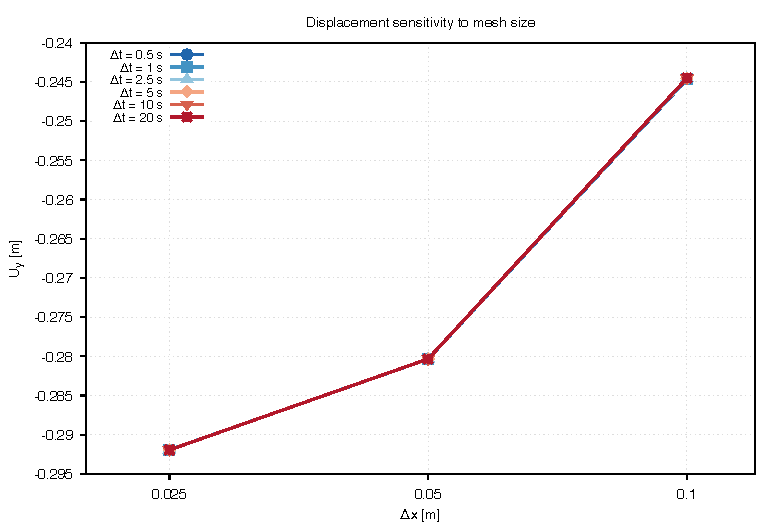
\includegraphics[width=0.48\textwidth]{simulationData/cavityFlexibleBottom/Uy_vs_DeltaX}
        \label{fig:cavity_Uy_vs_DeltaX}
    }
    \hfill
    \subfigure[Vertical resultant interface force.]{
        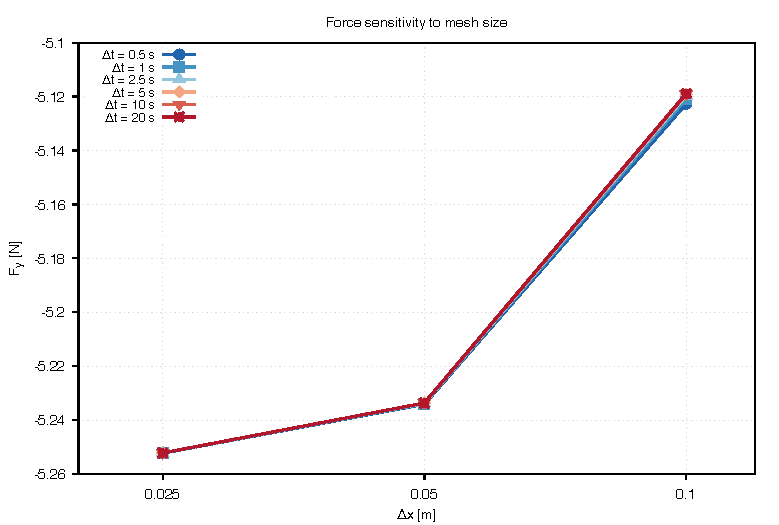
\includegraphics[width=0.48\textwidth]{simulationData/cavityFlexibleBottom/Fy_vs_DeltaX}
        \label{fig:cavity_Fy_vs_DeltaX}
    }

    \caption{Mesh and pseudo-time-step sensitivity of the steady-state solution for Case~1. The displacement and force predictions are primarily controlled by the mesh spacing, while the influence of the pseudo-time-step size is comparatively small for cases that reach the prescribed steady-state criterion.}
    \label{fig:cavity_solution_sensitivity}
\end{figure}

The computational cost associated with the same set of simulations is shown in Figure~\ref{fig:cavity_cost_sensitivity}. The wall-clock time increases with problem size, as expected, but the dependence on pseudo-time-step size is not monotonic. In particular, the smallest pseudo-time steps require many increments to reach steady state, while excessively large pseudo-time steps do not necessarily accelerate convergence. Instead, larger pseudo-time steps can lead to a longer pseudo-time interval before the automatic steady-state criterion is satisfied, increasing the total wall-clock time. For this case, an intermediate pseudo-time-step size gives the best overall efficiency.

\begin{figure}[htbp]
    \centering

    \subfigure[Wall-clock time.]{
        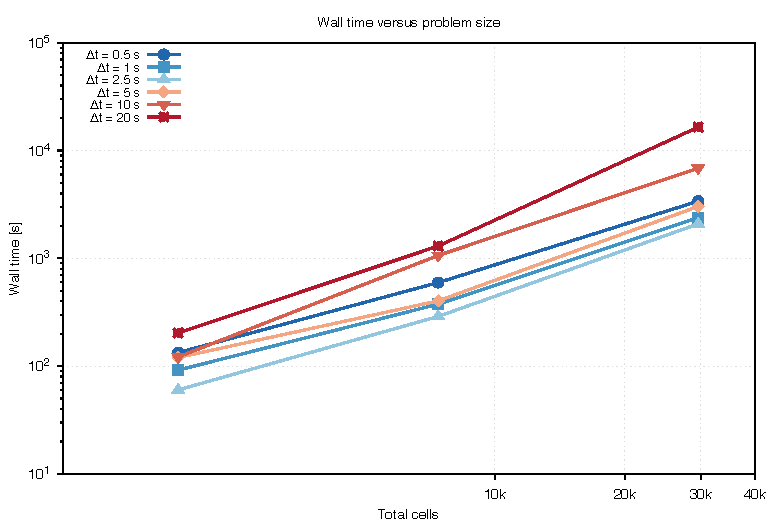
\includegraphics[width=0.48\textwidth]{simulationData/cavityFlexibleBottom/WallTime_vs_Cells}
        \label{fig:cavity_walltime_vs_cells}
    }
    \hfill
    \subfigure[Maximum memory usage.]{
        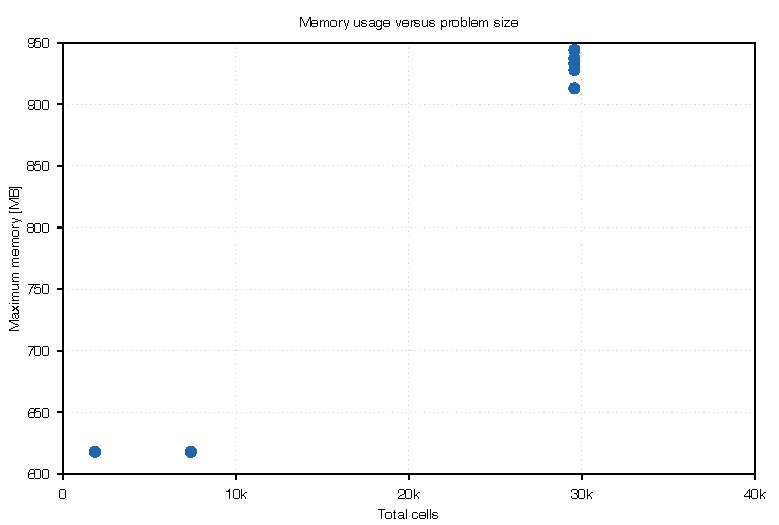
\includegraphics[width=0.48\textwidth]{simulationData/cavityFlexibleBottom/Memory_vs_Cells}
        \label{fig:cavity_memory_vs_cells}
    }

    \caption{Computational cost for Case~1 as a function of total cell count and pseudo-time-step size. The wall-clock time exhibits an optimum with respect to pseudo-time-step size: smaller values require more time steps, whereas larger values delay satisfaction of the automatic steady-state criterion. The memory usage is governed primarily by the total number of cells and is largely insensitive to the pseudo-time-step size.}
    \label{fig:cavity_cost_sensitivity}
\end{figure}

The existence of an optimal pseudo-time-step size can be understood from the competing effects that determine the total cost. Reducing $\Delta t$ improves the smoothness of the pseudo-transient evolution and tends to produce robust convergence to the steady state, but increases the number of time steps required. Conversely, increasing $\Delta t$ reduces the number of nominal time increments but can degrade the effectiveness of the pseudo-transient relaxation. In such cases, the monitored displacement and force may approach their final values more slowly, or exhibit small non-monotonic changes that delay the satisfaction of the steady-state criterion. Hence, the total wall-clock time is minimised by an intermediate value of $\Delta t$, rather than by the largest stable value.

The maximum memory usage, shown in Figure~\ref{fig:cavity_memory_vs_cells}, is primarily a function of the total number of fluid and solid cells. Unlike the wall-clock time, it shows little dependence on the pseudo-time-step size. This behaviour is expected for the present monolithic formulation, since the memory footprint is dominated by the storage of the coupled fields, linear-system data structures, and preconditioning objects, all of which are determined mainly by the number of degrees of freedom rather than by the pseudo-time-step size.


%- accuracy => show we get the same results as partitioned
%
%- time and memory => partitioned vs monolithic
%
%- time step effect => maybe show greater robustness as time step size is increased
%
%- [maybe other case] => show effect of preconditioner


%%--------------------------------------------------------------------------------------------------------------------%%
\subsection{Case 2: Three-dimensional flexible tube} \label{sec:case2}
%%--------------------------------------------------------------------------------------------------------------------%%
Case 2 is based on the solids4foam \texttt{3dTube} fluid-solid interaction tutorial. This benchmark extends the previous two-dimensional setting to a fully three-dimensional internal-flow problem in which fluid pressure and shear loads induce deformation of a compliant tube wall. It is selected to evaluate the solver's robustness under 3D coupling, increased system size, and stronger geometric nonlinearity in the structural response.

The test is run in transient mode with incompressible flow and finite-strain solid mechanics, using the same monolithic coupling strategy as Case 1. The principal outputs are the time evolution of pressure drop, wall displacement at selected monitoring locations, and integrated fluid-solid interface forces. Additional post-processing includes deformed-shape visualisation and final-time velocity and stress fields for qualitative comparison against the tutorial behaviour.

\begin{figure}[htbp]
	\centering
	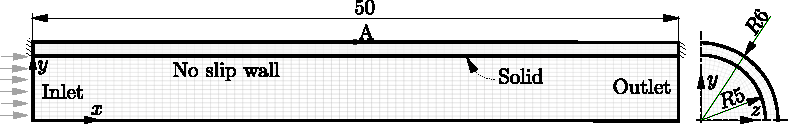
\includegraphics[scale=1]{figures/3dTube-geometry}
	\caption{Case 2 setup (\texttt{3dTube} benchmark): geometry and base mesh (dimensions are in mm).}
	\label{fig:HronTurek3_geom}
\end{figure}

%%--------------------------------------------------------------------------------------------------------------------%%
\subsection{Case 3: Flexible beam in cross-flow} \label{sec:case3}
%%--------------------------------------------------------------------------------------------------------------------%%
Case 3 is based on the solids4foam \texttt{beamInCrossFlow} tutorial, where an initially upright flexible beam undergoes flow-induced deformation in an external cross-flow configuration. Compared with Cases 1--2, this setup emphasises wake--structure interaction and large interface motion in an open-flow domain.

This case is used to assess stability and convergence of the monolithic algorithm for strongly coupled FSI with potentially oscillatory dynamics. The reported quantities are the tip-displacement history of the beam, the drag/lift forces on the structure, and representative flow-field contours. Where relevant, frequency content of the displacement signal is also analysed to characterise the coupled response.


%%--------------------------------------------------------------------------------------------------------------------%%
\subsection{Case 4: Hron--Turek FSI3 benchmark} \label{sec:case4}
%%--------------------------------------------------------------------------------------------------------------------%%
Case 4 follows the solids4foam \texttt{HronTurekFsi3} tutorial, a widely used benchmark for validating partitioned and monolithic FSI methods. The configuration consists of channel flow past a cylinder with an attached flexible flag-like structure, producing periodic structural deformation coupled with unsteady vortex shedding.

To facilitate comparison with established literature, the primary metrics are the displacement of the beam tip and the force coefficients over time. Mean values, oscillation amplitudes, and characteristic frequencies are extracted after initial transients. This benchmark provides a stringent test of accuracy and robustness for coupled fluid--structure dynamics.

\begin{figure}[htbp]
	\centering
	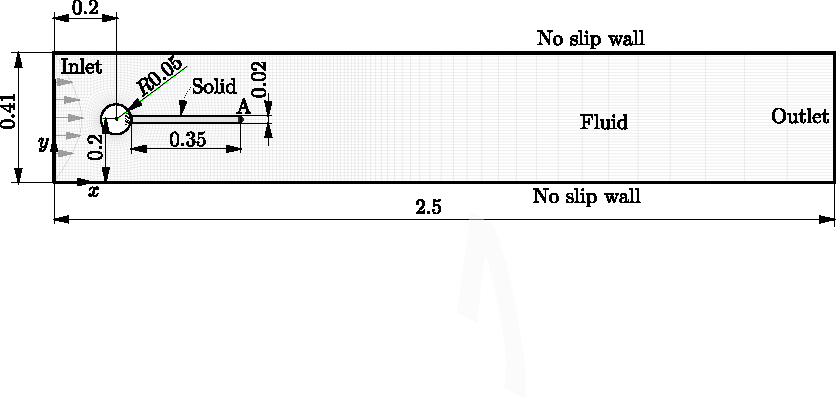
\includegraphics[scale=1]{figures/HronTurek3-geometry}
	\caption{Case 4 setup (Hron--Turek FSI3 benchmark): geometry and base mesh.}
	\label{fig:HronTurek3_geom}
\end{figure}

%%--------------------------------------------------------------------------------------------------------------------%%
\subsection{Case 5: Perpendicular flap (preCICE tutorial)} \label{sec:case5}
%%--------------------------------------------------------------------------------------------------------------------%%
Case 5 is based on the preCICE tutorial \texttt{perpendicular flap} case (fluid-solid interaction). This example is included to broaden the assessment to a benchmark frequently used in coupling-framework studies and to provide a cross-ecosystem reference beyond solids4foam-native tutorials.

The scenario features flow around a flexible flap mounted perpendicular to the incoming stream, generating coupled deflection and force oscillations. For this case, the same reporting strategy is adopted: time histories of flap-tip displacement, resultant interface forces, and representative flow/solid fields at selected times. Where feasible, key trends are compared qualitatively with the tutorial reference behaviour.

\begin{figure}[htbp]
	\centering
	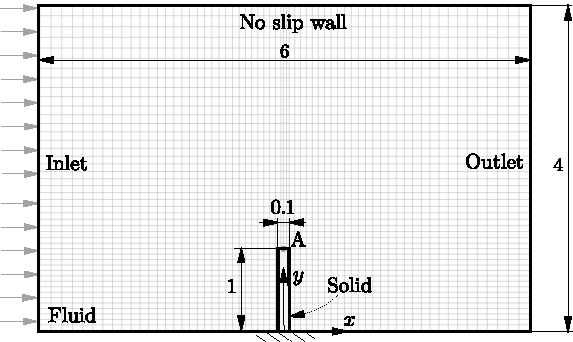
\includegraphics[scale=1]{figures/perpendicularFlap-geometry}
	\caption{Case 5 setup (perpendicular flap): geometry and base mesh.}
	\label{fig:cavity_geom}
\end{figure}

%%--------------------------------------------------------------------------------------------------------------------%%
\subsection{Case 6: Temporal-accuracy benchmark (elastic half-cylinder in channel)} \label{sec:case6}
%%--------------------------------------------------------------------------------------------------------------------%%
Case 6 is based on the user-provided benchmark screenshot (Section 6.7.1: \emph{Numerical Assessment of Temporal Accuracy}). The problem is a two-dimensional incompressible flow in a channel containing an elastic semi-cylinder attached to the lower wall. The computational domain is rectangular, $[0,5] \times [-0.5,1]$, and the semi-cylinder has radius $r=0.1$ with centre at $\boldsymbol{x}^c=(1.5,-0.5)$.

A time-ramped inlet velocity is prescribed at the left boundary,
\begin{equation}
\boldsymbol{u}^{in}=(U(y,t),0,0), \qquad U(y,t)=g(t)\,(1+2y)(1-y),
\end{equation}
with
\begin{equation}
 g(t)=
 \begin{cases}
 0, & t \le 0, \\
 1-\cos\!\left(\frac{\pi}{2}t\right), & t\in(0,2], \\
 1, & t>2.
 \end{cases}
\end{equation}
No-slip conditions are imposed on rigid walls, and a traction-free condition is applied at the outlet.

The constitutive parameters reported in the benchmark are: solid Young's modulus $E^s=10^5$, Poisson's ratio $\nu^s=0.4$, and density $\rho^s=500$; fluid density and kinematic viscosity are $\rho^f=1$ and $\nu^f=1$, respectively. Following the benchmark setup, temporal convergence is assessed using $\Delta t=1/40$, $1/80$, $1/120$, and $1/160$, with a reference solution computed at $\Delta t=2\times 10^{-5}$.

\begin{figure}[htbp]
	\centering
	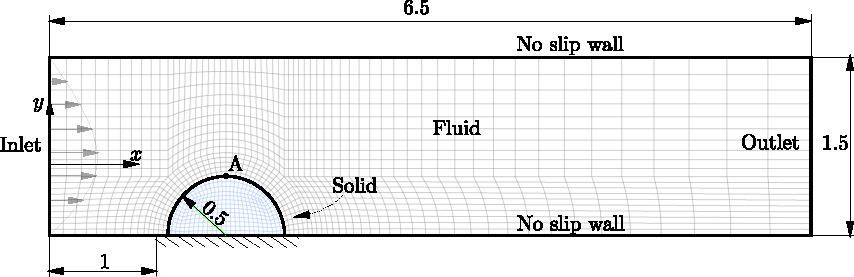
\includegraphics[scale=1]{figures/blobInTreacle-geometry}
	\caption{Case 6 setup (elastic half-cylinder in channel): geometry and base mesh (dimensions are in \hl{check}).}
	\label{fig:elasticHalfCylInChannel_geom}
\end{figure}



The error metric is the interface-displacement error in the streamwise direction, evaluated in the $L_2$ norm over the interface points,
\begin{equation}
\|error(\theta)\| = \| (\varphi(X,1)_{\Delta t=2\times 10^{-5}} - \varphi(X,1)_{\Delta t}) \|_{L_2}, \quad \forall\,X\in\Gamma,
\end{equation}
where $\theta=(1,0)$ denotes the positive $x$-direction. This case is used to verify the expected second-order temporal accuracy of the quasi-monolithic formulation.


%%--------------------------------------------------------------------------------------------------------------------%%
\subsection{Case 7: FSI accuracy assessment (block with flexible tail)} \label{sec:case7}
%%--------------------------------------------------------------------------------------------------------------------%%
Case 7 considers a block-with-flexible-tail configuration in cross-flow (extracted from the provided benchmark material). The setup is used to assess coupling accuracy through mesh refinement.

Extracted model data are: fluid density $\rho_f = 1.18\times 10^{-3}\,\mathrm{g\,cm^{-3}}$, fluid dynamic viscosity $\mu_f = 1.82\times 10^{-4}\,\mathrm{g\,cm^{-1}\,s^{-1}}$, tail density $\rho_s = 2.0\,\mathrm{g\,cm^{-3}}$, Young's modulus $E = 2.0\times 10^{6}\,\mathrm{g\,cm^{-1}\,s^{-2}}$, and Poisson's ratio $\nu = 0.35$. The inlet speed is $u_{in}=31.5\,\mathrm{cm\,s^{-1}}$.

The extracted geometry/boundary layout indicates a channel of height $12\,\mathrm{cm}$ with slip conditions on top and bottom walls and an outflow condition at the right boundary. The rigid block is followed by a thin flexible tail with annotated thickness $0.06\,\mathrm{cm}$.

\hl{IVAN comment: case geometry figure is the same as for case 8 (under assumption that we use the same mesh - which we can)}


%%--------------------------------------------------------------------------------------------------------------------%%
\subsection{Case 8: Three-dimensional block with flapping plate} \label{sec:case8}
%%--------------------------------------------------------------------------------------------------------------------%%
Case 8 is a three-dimensional extension with a flapping plate attached to a block (extracted from the provided benchmark material). The reference describes both top and side views and reports a multi-mesh study for convergence assessment.

Extracted fluid properties are again $\rho_f = 1.18\times 10^{-3}\,\mathrm{g\,cm^{-3}}$ and $\mu_f = 1.82\times 10^{-4}\,\mathrm{g\,cm^{-1}\,s^{-1}}$. Two plate material settings are described (stiffer and more flexible variants), with Poisson's ratio $\nu=0.35$ reported for both. The top-view dimensions shown in the source are $4\,\mathrm{cm}$--$3\,\mathrm{cm}$--$4\,\mathrm{cm}$ in the transverse direction.

In this manuscript, Case 8 is used as a 3D accuracy/robustness test with pronounced fluid-structure motion and higher computational cost than the 2D extracted benchmarks.

\begin{figure}[htbp]
	\centering
	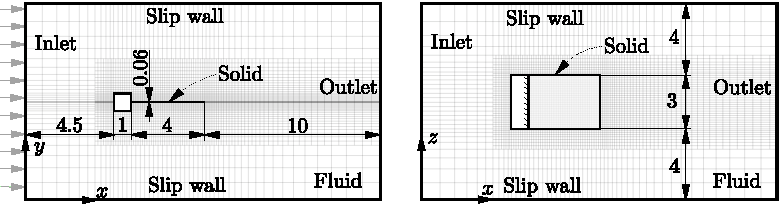
\includegraphics[scale=1]{figures/foilInWind-geometry}
	\caption{Case 8 setup (three-dimensional block with flapping plate): geometry and base mesh in side and top view (dimensions are in cm).}
	\label{fig:case8_schematic}
\end{figure}
%%%%%%%%%%%%%%%%%%%%%%%%%%%%%%%%%%%%%%%%%%%%%%%%%%%%%%%%%%%%%%%%%%
\section{Verification methodology}\label{sec:verification_methodology}
%%%%%%%%%%%%%%%%%%%%%%%%%%%%%%%%%%%%%%%%%%%%%%%%%%%%%%%%%%%%%%%%%%
% Evidence base: paper-data/benchmark_inventory.md, paper-data/benchmarks.yaml
% and the verification/ directories of the solids4foam development branch.

Code verification asks whether the discrete equations are solved correctly and whether the discretisation error vanishes at the expected rate; it does not ask whether the governing equations describe a physical system~\citetodo{Roache 1998, Verification and Validation in Computational Science and Engineering; Oberkampf \& Roy 2010}.
For a partitioned or monolithic fluid--structure interaction (FSI) calculation, the difference between a computed quantity $f$ and the exact solution of the stated mathematical problem, $f_\mathrm{exact}$, contains at least three contributions,
\begin{equation}
	f - f_\mathrm{exact} = \varepsilon_h + \varepsilon_{\Delta t} + \varepsilon_\mathrm{it},
	\label{eq:error_decomposition}
\end{equation}
namely the spatial discretisation error $\varepsilon_h$ (fluid, solid and, in ALE form, the fluid-mesh motion), the temporal discretisation error $\varepsilon_{\Delta t}$, and the iterative error $\varepsilon_\mathrm{it}$ left by incomplete convergence of the interface coupling iterations and of the field solvers within them.
A comparison with a benchmark value is informative only if each of these contributions is controlled, and only if the error of the benchmark value itself is known to be smaller than the differences being interpreted.
Many FSI benchmarks in current use do not meet the second condition, and this section sets out how the present paper distinguishes the cases.

Throughout, three notions are kept separate:
(i) a \emph{benchmark problem}, i.e.\ a precisely defined initial--boundary-value problem;
(ii) a \emph{published benchmark value}, i.e.\ a number or curve reported for that problem by one or more groups; and
(iii) a \emph{trustworthy verification reference}, i.e.\ a value whose own error is known to be small compared with the discretisation errors under study.
A widely used benchmark problem does not by itself provide (iii).

\todo{Section~\ref{sec:numerical_methods} currently describes the quasi-monolithic solver of the parent paper. All results in Sections~\ref{sec:benchmark_suite}--\ref{sec:cross_benchmark} were obtained with partitioned coupling: interface quasi-Newton with inverse least-squares (IQN-ILS)~\citep{Degroote2009}, Robin--Neumann coupling with a Robin condition for pressure~\citep{Tukovic2018b}, and Aitken under-relaxation~\citep{kuttler2008fixed}, in the solids4foam toolbox~\citep{Cardiff2025}. A concise description of these procedures, the fluid (\texttt{pimpleFluid}) and solid solvers, and the time schemes (\texttt{backward}, i.e.\ BDF2, unless stated) is required in Section~\ref{sec:numerical_methods}.}

%%%%%%%%%%%%%%%%%%%%%%%%%%%%%%%%%%%%%%%%%%%%%%%%%%%%%%%%%%%%%%%%%%
\subsection{Reference-solution hierarchy}\label{sec:ref_hierarchy}
%%%%%%%%%%%%%%%%%%%%%%%%%%%%%%%%%%%%%%%%%%%%%%%%%%%%%%%%%%%%%%%%%%

Each benchmark is assigned a reference category according to the quality of the reference against which it is compared (Table~\ref{tab:ref_hierarchy}).
The category describes the reference, not the benchmark problem and not the quality of the present calculations.

\begin{table}[htbp]
	\centering
	\small
	\setlength{\tabcolsep}{4pt}
	\caption{Reference-solution hierarchy used in this paper. The case assignments are discussed in Section~\ref{sec:benchmark_suite}.}
	\label{tab:ref_hierarchy}
	\begin{tabular}{p{1.4cm}p{6.6cm}p{5.4cm}}
		\toprule
		Category & Definition & Cases \\
		\midrule
		A & Analytical or semi-analytical solution of the stated continuum problem; any numerical error of its own (e.g.\ collocation) controlled to near round-off. & ringAddedMass, womersleyTube \\
		B & Independently computed numerical solution of the \emph{same} problem, by a different code, accompanied by its own convergence evidence. & collapsibleChannel (oomph-lib), Hron--Turek FSI1 (Featflow, six levels) \\
		C & Classical published benchmark value whose own discretisation error is only partly quantified. & Hron--Turek FSI2, FSI3 (Featflow level 4); beamInCrossFlow, original form \\
		C-weak & As C, but digitised from figures, single-mesh, mutually inconsistent, preprint-only, or from the same code lineage as the code under test. & 3dTube, mokLidDrivenCavity, cavityFlexibleBottom, beamInCrossFlow modified form, blobInTreacle \\
		\bottomrule
	\end{tabular}
\end{table}

Agreement with a category-A reference measures the total error directly.
Agreement with a category-B reference measures it up to the stated reference uncertainty, and is interpreted only where the difference exceeds that uncertainty.
Agreement with a category-C or C-weak reference is reported, but is not used as evidence of convergence; for these cases the primary verification evidence is self-convergence (below), and the comparison with published values is treated as a statement about the published values as much as about the present results.
References computed with earlier versions of the same code family~\citep{Tukovic2018} are explicitly classed as C-weak whatever their resolution, because they share discretisation choices with the code under test and cannot expose common-mode errors.

Two further distinctions are maintained throughout.
First, \emph{self-convergence}, i.e.\ the convergence of a sequence of solutions of one code towards its own limit, demonstrates that the discretisation is consistent and that the asymptotic range has been reached, but not that the limit is the correct one; it is not external verification.
Second, agreement between two coupling algorithms applied to the same discretisation (e.g.\ IQN-ILS and Robin--Neumann) is an internal consistency check on the iterative error and on the implementation of the coupling. It is not an independent reference, since both algorithms converge to the same discrete problem and share its discretisation error.
The Robin--Neumann scheme modifies the discrete interface condition~\citep{Tukovic2018b}; where this matters (Section~\ref{sec:fsi23}) the two couplings are not expected to agree to the coupling tolerance.

%%%%%%%%%%%%%%%%%%%%%%%%%%%%%%%%%%%%%%%%%%%%%%%%%%%%%%%%%%%%%%%%%%
\subsection{Spatial, temporal and iterative convergence}\label{sec:convergence_method}
%%%%%%%%%%%%%%%%%%%%%%%%%%%%%%%%%%%%%%%%%%%%%%%%%%%%%%%%%%%%%%%%%%

\paragraph{Refinement studies.}
Mesh studies refine the fluid and solid meshes together by a constant ratio $r$ (normally $r=2$ in each in-plane direction), with matching interface discretisations.
Unless stated otherwise the time step is reduced in proportion to the cell size so that the Courant number is unchanged; such a study measures the combined space--time error, and is identified as such.
Separate time-step studies are performed on a fixed mesh.
Where the mesh study is run at a fixed time step, the time error common to all levels cancels in the successive differences used for the observed order but not in the error against a reference; this is noted wherever it is significant (Section~\ref{sec:womersley}).

\paragraph{Observed order.}
For three solutions $f_1$, $f_2$, $f_3$ (fine to coarse) with constant refinement ratio $r$, the observed order is computed from successive differences,
\begin{equation}
	p = \frac{\ln\left[(f_3 - f_2)/(f_2 - f_1)\right]}{\ln r},
	\label{eq:observed_order}
\end{equation}
which requires no reference and is the primary self-convergence measure.
When an exact reference is available, the order of the error itself, $p = \ln(e_2/e_1)/\ln r$ with $e_i = |f_i - f_\mathrm{exact}|$, is also reported.
For category-B and C references, an \emph{apparent} order is sometimes computed in the same way with $f_\mathrm{ref}$ in place of $f_\mathrm{exact}$; this is meaningful only while $|f_1 - f_\mathrm{ref}|$ is large compared with the reference uncertainty, and two-level apparent orders are labelled as such.
An observed order is regarded as evidence of asymptotic convergence only when it is close to the formal order of the scheme (two in space and time for the methods used here) and stable across at least three levels; orders far above or below the formal value, or non-monotone sequences, indicate a pre-asymptotic regime or competing error sources.

\paragraph{Richardson extrapolation.}
Where three levels show an observed order consistent with the formal order, a Richardson estimate
\begin{equation}
	f_\mathrm{RE} = f_1 + \frac{f_1 - f_2}{r^{p} - 1}
	\label{eq:richardson}
\end{equation}
is used to quantify the remaining discretisation error of the finest solution~\citetodo{Richardson 1911; Roache 1998}.
It is used in this paper only where indicated, and never to promote a non-asymptotic sequence into a converged value.
\todo{Decide whether to report a grid-convergence index (GCI) with a safety factor~\citetodo{Roache 1994/1998} for the self-convergence cases, or to keep Richardson estimates only. The current evidence base does not tabulate GCIs.}

\paragraph{Iterative and coupling errors.}
In a partitioned calculation the interface iterations at each time step are stopped when a coupling residual falls below a tolerance (\texttt{outerCorrTolerance} for the IQN-ILS and Aitken procedures; displacement, pressure-change and leakage-flux residuals for Robin--Neumann), and the fluid and solid linear and nonlinear solvers have their own tolerances.
The resulting iterative error must be small compared with the discretisation error being measured, otherwise refinement studies converge towards a tolerance floor rather than to the continuum solution.
The direct test is a tolerance sweep at fixed discretisation; the indirect test is a comparison of two coupling algorithms.
As discussed in Section~\ref{sec:iterative_errors}, only a minority of the present cases contain a systematic tolerance sweep, and this is identified as a gap in the current evidence.

%%%%%%%%%%%%%%%%%%%%%%%%%%%%%%%%%%%%%%%%%%%%%%%%%%%%%%%%%%%%%%%%%%
\subsection{Quantities of interest and error measures}\label{sec:qoi}
%%%%%%%%%%%%%%%%%%%%%%%%%%%%%%%%%%%%%%%%%%%%%%%%%%%%%%%%%%%%%%%%%%

\paragraph{Choice of quantities.}
Each benchmark is assessed through a small set of quantities of interest (QoIs) that are defined unambiguously and are computable from both the present results and the reference: point displacements, integrated interface forces, natural frequencies, and, for the analytical references, complex amplitudes (amplitude and phase) of flow rate, wall displacement and the complex wave number.
Displacement-type, force-type and phase-type quantities are reported separately, because they need not converge at the same rate.
Point displacements integrate the solution over the structure and are typically the best-behaved QoIs; integrated forces depend on near-wall pressure and velocity gradients and therefore on the boundary-layer resolution; and phase, attenuation and lift-amplitude quantities depend on small differences between larger quantities.
The cross-benchmark consequences of this are collected in Section~\ref{sec:qoi_dependence}.

\paragraph{Error measures.}
Errors are reported as relative differences, $(f - f_\mathrm{ref})/|f_\mathrm{ref}|$, except where the reference value is near zero, in which case the error is normalised by a characteristic amplitude (e.g.\ the peak displacement for the collapsible-channel history, Section~\ref{sec:collapsible}).
Phase errors are reported in radians.
Comparisons with published curves digitised from figures carry the extraction uncertainty of the digitisation, which is stated with each such reference.

\paragraph{Periodic and transient quantities.}
For time-periodic responses the comparison is made on statistics over a window of complete periods after the start-up transient has decayed, with the periodicity of the window checked explicitly (the change between successive periods must be small compared with the reported errors).
For a forced periodic response with a known frequency, the complex Fourier coefficient at the forcing frequency is compared with the exact complex amplitude (womersleyTube).
For self-excited oscillations (Hron--Turek FSI2 and FSI3), the phase is arbitrary and the comparison is made on the window mean, the amplitude (half the mean peak-to-peak range) and the frequency, following the convention of~\citet{Turek2006}.
Free-vibration frequencies are obtained from zero crossings (ringAddedMass).
Transient benchmarks are compared on characteristic events (first trough, first peak, arrival time of a wavefront) as well as on full histories.

\paragraph{Reproducibility and machine-readable outputs.}
Every case in Section~\ref{sec:benchmark_suite} is accompanied in solids4foam~\citep{Cardiff2025} by an opt-in verification driver (\texttt{Allverify}) that is separate from the regression tests.
Each driver runs copies of the tutorial case under mesh, time-step and coupling variations, extracts the QoIs, and writes tabulated results (CSV) and a summary; reference values are stored in machine-readable files (JSON or CSV) that record, for each value, its source, figure or table, and extraction method; and the driver exits with a non-zero status unless every acceptance check passes.
Several drivers also record the OpenFOAM version and a fingerprint of the solver executable and libraries, and reuse a previous run only if these and the case-file hashes match.
These features are described further in Section~\ref{sec:infrastructure}.
\todo{State the exact solids4foam commit(s) and OpenFOAM version(s) used for every result reported. The current evidence was recorded on OpenFOAM-v2412 (ringAddedMass, womersleyTube, collapsibleChannel, Hron--Turek, 3dTube, mokLidDrivenCavity) and v2512 (cavityFlexibleBottom, blobInTreacle, beamInCrossFlow coupling checks), on macOS and Linux; see paper-data/manuscript\_todos.md. Plan a Zenodo archive of case set-ups, drivers, raw CSV outputs and reference files.}

%%%%%%%%%%%%%%%%%%%%%%%%%%%%%%%%%%%%%%%%%%%%%%%%%%%%%%%%%%%%%%%%%%
\section{Verification benchmark suite}\label{sec:benchmark_suite}
%%%%%%%%%%%%%%%%%%%%%%%%%%%%%%%%%%%%%%%%%%%%%%%%%%%%%%%%%%%%%%%%%%
% Every number in this section is traceable to paper-data/benchmark_inventory.md
% / benchmarks.yaml, which cite the solids4foam development-branch
% verification READMEs, reference JSON/CSV files and PR descriptions
% (inventory commit 7c928c55; no FSI tutorial changes up to c706be68).
% Values marked (derived) in comments were computed in the inventory from
% tabulated values; values marked (read from plot) are approximate.

The benchmarks are grouped by the quality of their reference (Table~\ref{tab:ref_hierarchy}) rather than by geometry or regime: problems with exact references (Section~\ref{sec:exact_refs}), problems with independently converged numerical references (Section~\ref{sec:independent_refs}), classical benchmarks whose published values are re-examined (Section~\ref{sec:classical}), three-dimensional problems of increasing geometric complexity (Section~\ref{sec:threeD}), and an additional transient problem (Section~\ref{sec:additional}).
Table~\ref{tab:suite_overview} summarises the suite and the verification evidence currently available for each case.
All calculations use the cell-centred finite volume fluid and solid solvers of solids4foam~\citep{Cardiff2025} with partitioned coupling; the second-order \texttt{backward} (BDF2) time scheme is used unless stated.

\begin{table}[htbp]
	\centering
	\footnotesize
	\setlength{\tabcolsep}{3pt}
	\caption{Overview of the benchmark suite and of the verification evidence currently available. Ref.: reference category (Table~\ref{tab:ref_hierarchy}). Mesh and $\Delta t$: number of levels in the refinement study (``scaled'' denotes $\Delta t$ reduced with $h$ in the mesh study, with no separate time study). Coupling: comparison of two coupling algorithms (IQN-ILS, Robin--Neumann (RN) or Aitken), or a coupling-tolerance sweep.}
	\label{tab:suite_overview}
	\begin{tabular}{llllllll}
		\toprule
		Case & Dim. & Regime & Solid & Ref. & Mesh & $\Delta t$ & Coupling \\
		\midrule
		ringAddedMass & 2-D & free vibration & small & A & 3 & 3 & IQN-ILS/RN \\
		womersleyTube & axisym. & periodic (forced) & small & A & 3 & 3 & IQN-ILS/RN \\
		collapsibleChannel & 2-D & transient & large & B & 4 (fluid) & 4 & IQN-ILS/RN; $\rho_s$ sweep \\
		Hron--Turek FSI1 & 2-D & steady & large & B & 2 & 2 & IQN-ILS/RN \\
		Hron--Turek FSI3 & 2-D & self-excited & large & C & 2 & scaled & IQN-ILS/RN \\
		Hron--Turek FSI2 & 2-D & self-excited & large & C & 2 & scaled & tolerance sweep \\
		3dTube & 3-D & transient pulse & small & C-weak & 2 & 4 & IQN-ILS/RN \\
		mokLidDrivenCavity & 2-D & periodic (forced) & large & C-weak & 4 & 3 & IQN-ILS/Aitken$^\dagger$ \\
		cavityFlexibleBottom$^\ast$ & 2-D & steady & large & C-weak & 3 & -- & none \\
		beamInCrossFlow$^\ast$ & 3-D & steady & small/large & C/C-weak & 4/5 & scaled & IQN-ILS/RN \\
		Hessenthaler$^\ast$ & 3-D & periodic & large & -- & -- & -- & -- \\
		blobInTreacle$^\ast$ & 2-D & trans.\,$\to$\,steady & large & C-weak & 4 & 4 & none \\
		\bottomrule
		\multicolumn{8}{l}{$^\ast$ Provisional (Sections~\ref{sec:cavity}, \ref{sec:beam}, \ref{sec:hessenthaler}, \ref{sec:blob}). $^\dagger$ Iteration counts only; no quantitative difference recorded.}
	\end{tabular}
\end{table}

\todo{Insert a figure panel with geometry sketches for ringAddedMass, womersleyTube, collapsibleChannel and mokLidDrivenCavity; geometry figures currently exist only for HronTurek, 3dTube, beamInCrossFlow, cavityFlexibleBottom and blobInTreacle (figures/*-geometry.pdf).}


%%%%%%%%%%%%%%%%%%%%%%%%%%%%%%%%%%%%%%%%%%%%%%%%%%%%%%%%%%%%%%%%%%
\subsection{Exact and semi-analytical reference problems}\label{sec:exact_refs}
%%%%%%%%%%%%%%%%%%%%%%%%%%%%%%%%%%%%%%%%%%%%%%%%%%%%%%%%%%%%%%%%%%

Both problems in this group are linear, small-amplitude problems whose exact solution is obtained from the continuum equations by a one-dimensional spectral (Chebyshev collocation) calculation that converges to near round-off.
They are therefore category A, and the total error of the coupled calculation can be measured directly, not inferred from self-convergence.
The collocation scripts are stored with the cases and are independent of solids4foam, although they were written by the same authors.

%%-------------------------------------------------------------------
\subsubsection{Ring added-mass problem}\label{sec:ring}
%%-------------------------------------------------------------------

\paragraph{Purpose.}
Added mass is the principal source of instability and slow convergence in partitioned FSI~\citep{Causin2005}.
Most benchmarks contain an added-mass effect of fixed, unquantified strength.
This problem isolates it: the fluid lowers the natural frequency of an elastic ring by an amount that linear theory gives exactly, and the strength of the effect is varied over two decades at fixed solid properties.

\paragraph{Problem.}
An elastic ring vibrates freely in its $n=2$ (ovalling) mode inside a fluid-filled rigid annulus (plane strain; a quarter of the domain is modelled with symmetry conditions).
The fluid is incompressible with $\nu_f = 10^{-7}\,\mathrm{m^2/s}$, i.e.\ effectively inviscid; the Stokes layer is deliberately not resolved.
The amplitude is approximately $5\times10^{-4}$ of the ring radius and the solid is modelled with linear geometry.
Three fluid densities give mass ratios $\mu = 0.101$, $1.008$ and $10.08$ (``weak'', ``moderate'', ``strong''), and a dry (in vacuo) run is made on each mesh.
\todo{Add a short parameter table (ring radii, thickness, $E$, $\nu$, $\rho_s$, outer wall radius) from the tutorial README, and the definition of $\mu$.}

\paragraph{Reference.}
The reference (category A) is the exact linear eigenvalue of a plane-strain continuum ring loaded by the exact potential-flow added-mass traction, computed by Chebyshev collocation with 24 intervals; refining the collocation changes the frequencies by approximately $5\times10^{-8}$.
The classical thin-ring frequency with the confined added mass of Brennen~\citetodo{Brennen 1982, NCEL report CR 82.010; not in bibliography} agrees with it to $O((h/a)^2)$ and serves as a check.
The exact dry frequency is $\omega_\mathrm{dry} = 2.555042\,\mathrm{rad/s}$, and the wet frequencies are $2.435615$, $1.804513$ and $0.768654\,\mathrm{rad/s}$ for the three levels.
A linearised viscous solution, also stored, shifts these by $-0.004\%$, $-0.026\%$ and $-0.073\%$, which bounds the effect of the small fluid viscosity.

\paragraph{Verification study.}
Frequencies are measured from zero crossings over four periods.
The mesh study uses refinement factors 1, 2 and 4 (solid $4\times48$ to $16\times192$ cells; fluid $12\times48$ to $48\times192$) at 100 steps per period, and the time-step study uses 25, 50 and 100 steps per period on the middle mesh.
Two solid discretisations are compared (the standard second-order residual and a cubic high-order residual), as are the IQN-ILS and Robin--Neumann couplings.
Table~\ref{tab:ring} gives representative results.

\begin{table}[htbp]
	\centering
	\small
	\setlength{\tabcolsep}{5pt}
	\caption{ringAddedMass: frequency error against the exact continuum solution and error of the wet/dry frequency ratio (high-order solid, IQN-ILS). Mesh: refinement factor; steps: time steps per period. Source: solids4foam \texttt{ringAddedMass/verification/README.md}.}
	\label{tab:ring}
	\begin{tabular}{lrrrrr}
		\toprule
		Level & Mesh & Steps & $\omega$ (rad/s) & Error in $\omega$ & Error in ratio \\
		\midrule
		dry & 1 & 100 & 2.55254 & $-0.098\%$ & -- \\
		dry & 4 & 100 & 2.55173 & $-0.129\%$ & -- \\
		dry & 2 & 25 & 2.50576 & $-1.929\%$ & -- \\
		strong ($\mu=10.08$) & 1 & 100 & 0.76843 & $-0.029\%$ & $+0.068\%$ \\
		strong & 2 & 100 & 0.76796 & $-0.090\%$ & $+0.021\%$ \\
		strong & 4 & 100 & 0.76770 & $-0.124\%$ & $+0.006\%$ \\
		strong & 2 & 25 & 0.75477 & $-1.806\%$ & $+0.125\%$ \\
		strong & 2 & 50 & 0.76552 & $-0.408\%$ & $+0.087\%$ \\
		\bottomrule
	\end{tabular}
\end{table}

\paragraph{Findings.}
\begin{itemize}
	\item \emph{Time.} The observed temporal orders of the frequency are 1.90, 1.92, 2.02 and 2.14 (dry, weak, moderate, strong), consistent with BDF2. Richardson extrapolation in time brings every frequency to within $+0.018\%$ of the exact value. The residual error of approximately $-0.13\%$ at 100 steps per period is therefore the phase error of the time scheme, not a coupling or spatial error.
	\item \emph{Space.} With the high-order solid the frequencies change by at most $0.06\%$ between meshes, too little to define a spatial order: the frequency is spatially converged on the coarsest mesh, and the slight growth of $|\text{error}|$ with refinement in Table~\ref{tab:ring} reflects the removal of a small spatial error that partly offsets the temporal one. The wet/dry ratio, in which the common time error cancels, converges at observed orders 1.77, 1.73 and 1.68 to $+0.001\%$, $+0.003\%$ and $+0.006\%$ on the finest mesh.
	\item \emph{Solid discretisation.} The standard second-order solid is $20.7\%$ too stiff in bending on the coarsest mesh and $1.6\%$ on the finest (observed order 1.66), whereas the high-order solid is within $0.13\%$ on every mesh. Nevertheless the wet/dry ratio of the two solids agrees to $0.003\%$ on the finest mesh: the added-mass coupling is verified independently of the accuracy of the solid discretisation.
	\item \emph{Coupling.} IQN-ILS and Robin--Neumann agree to $0.03\%$ in frequency. Mean coupling iterations per step are 2.99, 3.95 and 4.91 for IQN-ILS and 3.87, 4.85 and 12.29 for Robin--Neumann (weak to strong).
	\item \emph{Unresolved.} The IQN-ILS solutions lose amplitude at a rate that depends on the mesh and the added mass (up to $2.1\%$ per period on the coarsest mesh at the strong level, halving with each refinement), whereas the Robin--Neumann solutions are almost undamped ($\leq0.05\%$ per period on the middle mesh). The mechanism has not been identified. It does not affect the frequency at the reported precision.
\end{itemize}

\paragraph{Role in the suite.}
This is the only case with an exact reference and a controlled added-mass ratio spanning two decades.
Because dry and wet runs share the solid and time discretisations, the wet/dry ratio isolates the fluid--solid coupling from the solid and temporal errors.
The problem is inexpensive (the full study of 35 runs takes about 30\,min on 32 cores; the tutorial about 75\,s serial).
Its limitations are that viscous effects are, by design, not verified, and that only small-amplitude linear dynamics are tested.

%%-------------------------------------------------------------------
\subsubsection{Pulsatile compliant tube}\label{sec:womersley}
%%-------------------------------------------------------------------

\paragraph{Purpose.}
Pressure-wave propagation in a compliant vessel combines added mass, viscous attenuation and wall compliance, and is the canonical haemodynamic FSI configuration.
Womersley's analysis~\citetodo{Womersley 1955 Phil.\ Mag.; Womersley 1957 Phys.\ Med.\ Biol.} has been used to verify FSI codes before~\citetodo{Filonova et al.\ 2020, IJNMBE e3266}, usually in a thin-wall, long-wave form whose own modelling error is not negligible for a thick wall.

\paragraph{Problem.}
A harmonic pressure wave travels along an axisymmetric elastic tube (modelled as a $1^\circ$ wedge) of inner radius $R = 1\,\mathrm{m}$, wall thickness $h/R = 0.1$ and length $L = 15\,\mathrm{m}$, at Womersley number $\alpha = 5.01$ and mass ratio $\rho_s h/(\rho_f R) = 0.1$.
The wall is free to move axially (untethered).
The finite segment reproduces the infinite-tube solution because the exact travelling-wave data are imposed at both ends, so no reflection is generated, and the fields are initialised with the exact solution.
The wall radial displacement is approximately $5\times10^{-4}R$ and the peak velocity approximately $1.5\times10^{-3}$ of the wave speed, so the linear theory is appropriate and differences much below $10^{-3}$ are not expected to be meaningful.

\paragraph{Reference.}
The reference (category A) is the exact linear solution of the continuum problem: a thick linear-elastic cylinder (Chebyshev collocation, 16 intervals) coupled to the full linearised Navier--Stokes equations, with the complex wave number found from the frequency equation.
Collocation with 8 and 24 intervals agrees to approximately $10^{-11}$.
The solution reduces to Womersley's thin-wall equation, in the form of Filonova et al.\ (their Eq.~41), as $h/R\to0$, and agrees with the tethered long-wave limit to $2\times10^{-5}$.
The exact wave number is $k = 0.143978 - 0.020727\mathrm{i}\,\mathrm{m^{-1}}$, i.e.\ a wave speed of $0.872796\,\mathrm{m/s}$.
Womersley's thin-wall wave speed is $4.7\%$ higher for this wall thickness; using it as the reference would have hidden discretisation errors of the size studied here.

\paragraph{Verification study.}
The QoIs are the first Fourier coefficients at the forcing frequency, over the fifth and sixth periods, of: the axial velocity profile at $x = L/2$ (maximum error over the radius), the flow rate (amplitude and phase), the wall radial displacement at $L/2$ (amplitude and phase), and the wave speed and attenuation fitted to the pressure along the tube.
The mesh study refines all directions by factors 1, 2 and 4 (from 32 axial, 10 fluid-radial and 4 wall-radial cells) at 200 steps per period; the time-step study uses 50, 100 and 200 steps per period on the middle mesh; both use Robin--Neumann coupling.
IQN-ILS and Robin--Neumann are compared at 100 steps per period.
The change of the wall-displacement coefficient between the fifth and sixth periods is below $10^{-4}$ in every run.

\begin{table}[htbp]
	\centering
	\small
	\setlength{\tabcolsep}{5pt}
	\caption{womersleyTube: observed orders from successive differences (three levels) and finest-mesh errors against the exact solution (mesh factor 4, 200 steps per period). The profile mesh order is from its errors on the two finest meshes. Phases in radians. Source: solids4foam \texttt{womersleyTube/verification/README.md}.}
	\label{tab:womersley}
	\begin{tabular}{lrrr}
		\toprule
		Quantity & Mesh order & Time order & Finest-mesh error \\
		\midrule
		velocity profile (max.) & 2.06 & -- & $1.18\times10^{-3}$ \\
		flow-rate amplitude & 2.16 & 1.64 & $-7.15\times10^{-4}$ \\
		flow-rate phase & 1.92 & 1.84 & $1.5\times10^{-5}$ \\
		wall displacement amplitude & 2.15 & 1.71 & $8.57\times10^{-4}$ \\
		wall displacement phase & 0.97 & 1.74 & $-1.88\times10^{-3}$ \\
		wave speed & 2.48 & 1.29 & $8.93\times10^{-4}$ \\
		attenuation, $\mathrm{Im}(k)$ & 0.63 & 1.51 & $-4.47\times10^{-3}$ \\
		\bottomrule
	\end{tabular}
\end{table}

\paragraph{Findings.}
\begin{itemize}
	\item \emph{Space.} The velocity profile, flow rate, wall-displacement amplitude and wave speed converge at approximately second order in space (Table~\ref{tab:womersley}), and on the finest mesh agree with the exact solution to $0.12\%$ or better. The wall-displacement phase and the attenuation converge at only about first order, and the attenuation has the largest error, $-0.45\%$. Since $\mathrm{Im}(k)$ is only $14\%$ of $\mathrm{Re}(k)$, a given error in the fitted wave number is about seven times larger relative to the attenuation; the reason for the first-order phase convergence has not been established.
	\item \emph{Time.} The observed temporal orders are 1.29--1.84, \emph{below} the nominal second order of the BDF2 scheme that is used in both the fluid and the solid and in the interface-velocity condition. The cause has not been identified. Because the reference is exact, this finding is not an artefact of an imperfect reference: it is a property of the coupled discretisation (or of the start-up, see below) that a benchmark with a weaker reference could not have exposed.
	\item \emph{Start-up.} A transient of approximately $0.5\%$ in the wall displacement remains over the first period even though the fields are initialised exactly, and it \emph{grows} as the time step is reduced. One candidate is an inconsistency between the exact initial point displacements used to move the fluid mesh and the solid model's interpolation of its cell values. A start-up correction made elsewhere in the code for a different time scheme has been checked and does not apply to the \texttt{backward} scheme used here. Six periods are run and the last two are analysed to avoid contamination by this transient.
	\item \emph{Space--time interaction.} At 200 steps per period the temporal error is of the same size as the spatial error on the finest mesh. The successive-difference mesh orders cancel this common error, but the finest-mesh errors in Table~\ref{tab:womersley} contain it.
	\item \emph{Coupling.} IQN-ILS and Robin--Neumann agree to $3\times10^{-4}$ or better in every QoI (14.8 and 8.7 coupling iterations per step, respectively).
\end{itemize}

\todo{Do NOT remove or soften the sub-nominal temporal order. Planned diagnosis (paper-data/manuscript\_todos.md): time study on mesh factor 4 and at 400 steps per period; isolate the interface-velocity condition and the start-up transient. If the cause is found, report both the diagnosis and the corrected order; if not, retain the present statement as an open finding. Also note: the Robin--Neumann result moved by $0.26\%$ of amplitude between OpenFOAM-v2412 and v2512 (PR \#513 comment), which is larger than several of the finest-mesh errors in Table~\ref{tab:womersley} and must be resolved before the final numbers are fixed.}

\paragraph{Role in the suite.}
This is the only viscous, time-periodic, wave-propagation case with an exact reference, and the only axisymmetric case.
It complements ringAddedMass (inviscid, standing mode) and provides separate amplitude and phase QoIs.
Its central result for this paper is a negative one: an exact reference exposes a sub-nominal temporal order and a slow, first-order convergence of phase and attenuation that are not visible in the more widely used benchmarks.
Limitations: the tube wall is untethered, unlike Womersley's constrained tube, because a suitable mixed displacement--traction condition is not yet available for the solid solver used (solids4foam issue \#511); the high-order solid residual cannot be used on wedge meshes (issue \#512); the evidence was recorded on one OpenFOAM version and platform.


%%%%%%%%%%%%%%%%%%%%%%%%%%%%%%%%%%%%%%%%%%%%%%%%%%%%%%%%%%%%%%%%%%
\subsection{Independently resolved numerical benchmarks}\label{sec:independent_refs}
%%%%%%%%%%%%%%%%%%%%%%%%%%%%%%%%%%%%%%%%%%%%%%%%%%%%%%%%%%%%%%%%%%

The two problems in this group have no analytical solution, but have references computed with independent codes, discretisations and solution strategies, each with its own convergence evidence (category B).
Differences between the present results and the reference are interpreted only where they exceed the reference uncertainty.

%%-------------------------------------------------------------------
\subsubsection{Collapsible channel}\label{sec:collapsible}
%%-------------------------------------------------------------------

\paragraph{Purpose.}
A thin, very light elastic wall in a channel carrying internal flow combines strong added mass, bending-dominated large deformation and fluid-mesh motion.
Flow in collapsible channels is a classical FSI problem~\citetodo{Jensen \& Heil 2003, J.\ Fluid Mech.}~\citep{Heil2004, Heil2008}, and the strongly coupled internal-flow configuration is precisely where partitioned methods are least robust.

\paragraph{Problem.}
A two-dimensional channel with an elastic section of its upper wall (thickness $h/L = 0.005$) is subjected to a ramped external pressure; the wall collapses to approximately $21\%$ of the channel width at the first trough and then performs a damped oscillation of period approximately $0.8\,\mathrm{s}$, analysed to $t = 1.5\,\mathrm{s}$.
The flow has $Re = Re\,St = 50$ and is driven by an imposed pressure drop with Poiseuille inflow.
The solid is a total-Lagrangian St Venant--Kirchhoff continuum.
A small regularising wall density $\rho_s = \rho_f$ is used.

The problem is a \emph{modified} version of the published configuration of Jensen and Heil: the wall has no pre-stress ($\sigma_0 = 0$), $h/a = 1/20$, clamped ends, a pressure ramp and the regularising density.
The regularising density shifts the response by $0.28\%$ of the peak displacement relative to a massless wall.
These modifications are made so that the problem is well posed for a continuum solid and for partitioned coupling; the results therefore verify the code on this modified problem and do not reproduce the published values.

\paragraph{Reference and controlled model-form difference.}
The reference (category B) is computed with oomph-lib\citetodo{Heil \& Hazel 2006, oomph-lib}, a monolithic Newton finite element code, with Taylor--Hood (Q2Q1) or Crouzeix--Raviart (Q2P-1) fluid elements and a geometrically nonlinear Kirchhoff--Love \emph{beam} for the wall, using BDF2 for the fluid and a Newmark scheme for the beam.
The driver source is stored with the case, so the reference can be regenerated.
The converged reference is a Richardson extrapolation in time from $\Delta t = 0.003125$ and $0.0015625\,\mathrm{s}$; its uncertainty is approximately $0.3\%$ of the peak displacement, dominated by the oomph-lib spatial error (refinement levels 1 and 2 differ by $0.26\%$; the Richardson correction is $0.06\%$; the two fluid element types differ by less than $0.001\%$).

The comparison contains a deliberate, controlled \emph{model-form} difference: oomph-lib represents the wall as a geometrically nonlinear beam, whereas solids4foam resolves it as a two-dimensional continuum.
The difference is of order $h/L$; for the static deflection under the steady load it is $0.05\%$, which is used as an estimate of the model-form contribution.
A difference between the two solutions below approximately $0.3\%$ of the peak (reference uncertainty) plus this model-form contribution cannot be attributed to either code.

\paragraph{Verification study.}
The QoI is the vertical displacement history of the wall midpoint (and quarter points), with the first trough as a scalar summary.
Four studies are performed: a static wall test; a solid-discretisation comparison (cubic high-order versus linear least-squares reconstruction); a fluid-mesh study (four levels, 3\,200 to 51\,200 fluid cells, Robin--Neumann coupling, fixed $\Delta t = 0.00625\,\mathrm{s}$, compared with oomph-lib at the same $\Delta t$); and a time-step study ($\Delta t = 0.025$ to $0.003125\,\mathrm{s}$ on the coarsest fluid mesh).
The coupling study compares IQN-ILS and Robin--Neumann and maps the range of wall densities for which each completes, from $\rho_s/\rho_f = 0$ to 3.

\begin{figure}[htbp]
	\centering
	% Source: solids4foam development, tutorials/fluidSolidInteraction/collapsibleChannel/verification/reference/mesh_study_wallMid.png (PR #507).
	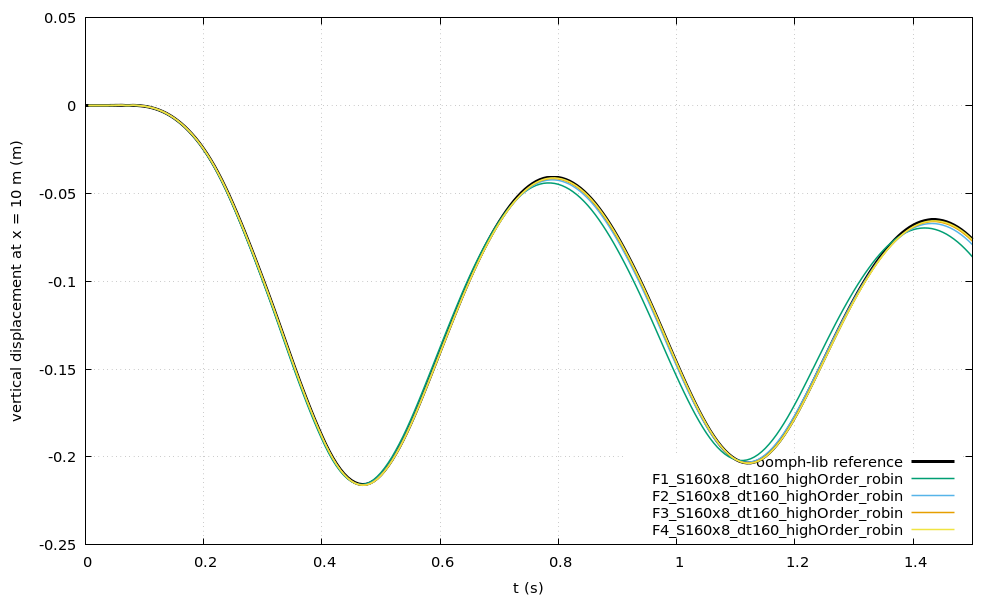
\includegraphics[width=0.85\textwidth]{figures/verification/collapsibleChannel_mesh_study_wallMid}
	\caption{collapsibleChannel: wall-midpoint vertical displacement for fluid-mesh levels F1--F4 (solid mesh $160\times8$, $\Delta t = 0.00625\,\mathrm{s}$, high-order solid, Robin--Neumann coupling) against the oomph-lib reference. Interim figure reproduced from the solids4foam verification output.}
	\label{fig:collapsible_mesh}
\end{figure}
\todo{Replace Figure~\ref{fig:collapsible_mesh} with a publication-quality version (legend labels, inset at first trough and second peak, error-versus-$h$ panel). The current PNG legend shows raw run identifiers.}

\paragraph{Findings.}
\begin{itemize}
	\item \emph{Static wall.} The cubic solid is within $0.25\%$ of the oomph-lib static deflection on all solid meshes and converges to a $0.05\%$ difference, the beam--continuum model-form difference. The linear-reconstruction solid has errors from $-16.7\%$ to $-0.22\%$ (approximately second order in the in-plane spacing).
	\item \emph{Solid in the coupled problem.} On the tutorial mesh the cubic solid contributes $0.44\%$ error, against $17.4\%$ for the linear reconstruction. For a thin bending-dominated wall the solid discretisation can thus dominate the FSI error unless a high-order or well-resolved solid is used.
	\item \emph{Fluid mesh.} The error against oomph-lib at the same $\Delta t$ falls from $4.65\%$ to $1.43\%$, $0.53\%$ and $0.50\%$ of the peak displacement (observed orders 1.7 and 2.4, then a floor) (Fig.~\ref{fig:collapsible_mesh}). The floor coincides with the reference uncertainty of approximately $0.3\%$ plus the model-form contribution; the finest-mesh first trough is $-0.21610\,\mathrm{m}$ against $-0.2160\,\mathrm{m}$ for the converged oomph-lib reference.
	\item \emph{Time step.} Successive differences of $4.56\%$, $1.33\%$ and $0.34\%$ give orders 1.8 and 2.0; oomph-lib itself shows 1.8 and 1.9 on the same sequence.
	\item \emph{Coupling.} IQN-ILS and Robin--Neumann agree to $0.08$--$0.23\%$ of the peak, but this gap does \emph{not} decrease with mesh refinement; it is of the size expected from the coupling tolerance and is therefore an iterative, not a discretisation, error. In the density sweep IQN-ILS fails to complete for part of the range, whereas Robin--Neumann completes for all $\rho_s/\rho_f \geq 1$.
\end{itemize}

\paragraph{Role in the suite.}
This is the strongest independent-code comparison in the suite: a regenerable monolithic finite element reference, with its own time-convergence and spatial-uncertainty estimate, for a large-deformation, strongly added-mass internal flow.
It also shows that once the discretisation error falls to approximately $0.5\%$, the reference uncertainty, the model-form difference and the coupling tolerance are all of comparable size, so that further agreement cannot be expected without tightening all three.
Limitations: the temporal error on the finer fluid meshes has not been measured separately; the mesh and time studies follow separate refinement paths; the high-order solid is serial only, and a 4-rank run with the linear-reconstruction solid gave an incorrect displacement that remains to be re-checked.

%%-------------------------------------------------------------------
\subsubsection{Hron--Turek FSI1}\label{sec:fsi1}
%%-------------------------------------------------------------------

\paragraph{Purpose.}
FSI1 is the steady, low-Reynolds-number member of the Turek--Hron family~\citep{Turek2006}: an elastic flag attached to a rigid cylinder in a channel at $Re = 20$.
It tests steady coupling with small loads and small (but geometrically nonlinear) deformation, and it has the best-converged published reference of the classical benchmarks.

\paragraph{Reference.}
The Featflow results for FSI1 are tabulated on six mesh levels (2+0 to 7+0, the finest with approximately $10^6$ elements); the spread across these levels is $0.73\%$ in $u_x$, $0.19\%$ in $u_y$, $0.14\%$ in drag and $0.26\%$ in lift.
The finest values ($u_x = 2.2705\times10^{-5}\,\mathrm{m}$, $u_y = 8.2088\times10^{-4}\,\mathrm{m}$, drag $14.2943\,\mathrm{N/m}$, lift $0.76375\,\mathrm{N/m}$) are therefore treated as an independently converged (category-B) reference.
\todo{Cite the Featflow table source precisely (Turek--Hron benchmark web pages / Turek et al.\ 2010 book chapter?)~\citetodo{Featflow FSI benchmark tables}; confirm that the six-level spread quoted is from that source.}

\paragraph{Verification study.}
The steady state is reached by pseudo-transient integration to $t = 30\,\mathrm{s}$.
Two mesh levels (1x and 2x; the 4x level is defined but has not been run) are compared with the Featflow finest level, and two time steps ($\Delta t = 0.025$ and $0.01\,\mathrm{s}$) are compared on the 1x mesh.
Steady IQN-ILS and Robin--Neumann solutions are compared, and the fluid solver tolerance is varied from $10^{-6}$ to $10^{-9}$.

\paragraph{Findings.}
On the 2x mesh the errors are $0.97\%$ in $u_x$, $4.64\%$ in $u_y$, $0.24\%$ in drag and $1.55\%$ in lift (1x: $u_y = 7.0426\times10^{-4}\,\mathrm{m}$; 2x: $7.8282\times10^{-4}\,\mathrm{m}$).
The two-level apparent orders against the Featflow finest level are 1.5--1.7.
The pseudo-time step changes $u_y$ and drag by $0.04\%$ and $u_x$ by $0.26\%$; the coupling algorithms agree to $0.01\%$; the fluid solver tolerance changes the steady values by at most $2\times10^{-4}$.
The transverse tip displacement $u_y$ is thus the slowest-converging QoI, even though the drag is already within $0.25\%$ on the 2x mesh.

\paragraph{Role in the suite.}
FSI1 is the cheapest category-B problem with large-deformation kinematics (1x: 781\,s serial; 2x: 3\,062\,s on 2 ranks) and is a natural first steady FSI check.
With only two levels, however, no reference-free order is available, and the apparent orders (1.5--1.7) are below the formal order; a third level is needed to establish whether the sequence is asymptotic.
\todo{Run the 4x level (estimated $>14$\,h on 3 ranks) to obtain a three-level, reference-free order for $u_y$. Without it, report FSI1 as ``converging towards the Featflow reference'' rather than ``verified to second order''.}


%%%%%%%%%%%%%%%%%%%%%%%%%%%%%%%%%%%%%%%%%%%%%%%%%%%%%%%%%%%%%%%%%%
\subsection{Classical FSI benchmarks revisited}\label{sec:classical}
%%%%%%%%%%%%%%%%%%%%%%%%%%%%%%%%%%%%%%%%%%%%%%%%%%%%%%%%%%%%%%%%%%

The benchmarks in this group are widely used, but their published values carry incompletely quantified error, are inconsistent between sources, or both.
For each, the present calculations are first established by self-convergence, and the comparison with the literature is then used to examine the published values themselves.

%%-------------------------------------------------------------------
\subsubsection{Hron--Turek FSI2 and FSI3}\label{sec:fsi23}
%%-------------------------------------------------------------------

\begin{figure}[htbp]
	\centering
	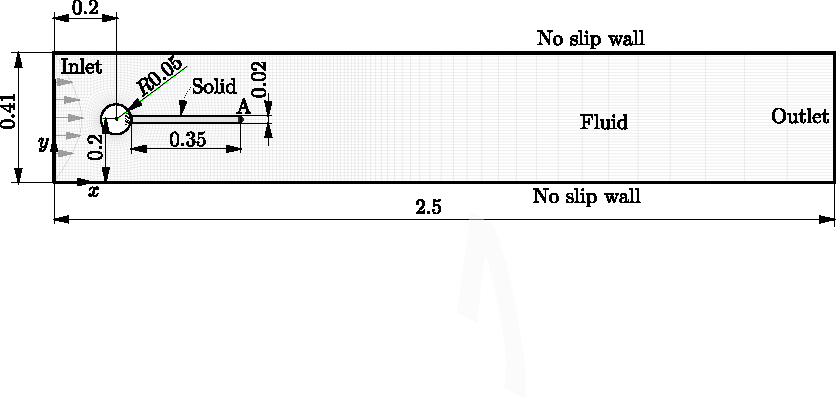
\includegraphics[scale=1]{figures/HronTurek3-geometry}
	\caption{Hron--Turek benchmark geometry (shown for FSI3; FSI1 and FSI2 share the geometry).}
	\label{fig:hronturek_geom}
\end{figure}

\paragraph{Purpose.}
FSI2 and FSI3 are the self-excited periodic members of the family~\citep{Turek2006} (Fig.~\ref{fig:hronturek_geom}).
FSI3 ($Re = 200$, $\rho_s = \rho_f$) tests a low mass ratio and a high-frequency vortex-induced oscillation of moderate amplitude ($u_y \approx \pm35\,\mathrm{mm}$); FSI2 ($Re = 100$, a heavier and softer flag) tests large-amplitude flapping ($u_y \approx \pm80\,\mathrm{mm}$) and the resulting distortion of the fluid mesh.

\paragraph{Reference and its ambiguity.}
The references are the Featflow level-4 tables (FSI3: $\Delta t = 0.00025\,\mathrm{s}$; FSI2: $\Delta t = 0.0005\,\mathrm{s}$).
For FSI2, the Featflow values change by $0.9$--$2.5\%$ between levels 3 and 4, so the reference itself is uncertain by approximately $1\%$; both cases are classed as category C.
The detailed Featflow tables differ from the summary values of~\citet{Turek2006} that are most often quoted (Table~\ref{tab:hronturek_ref}).
The largest difference is in the FSI3 drag amplitude ($22.66$ in the summary against $27.74\,\mathrm{N/m}$ in the table, $-18\%$); the summary frequencies are also rounded ($5.3$ against $5.46\,\mathrm{Hz}$ for FSI3 $u_y$; $2.0$ against $1.93\,\mathrm{Hz}$ for FSI2).
The present study uses the tables.
As a consistency check, the verification driver reproduces the tabulated statistics from the published Featflow time histories to within $0.7\%$ (FSI3; $1.1\%$ for the drag amplitude) and $0.3\%$ (FSI2).
A comparison with the summary values would misattribute an $18\%$ difference in FSI3 drag amplitude to the code under test.

\begin{table}[htbp]
	\centering
	\small
	\setlength{\tabcolsep}{5pt}
	\caption{Hron--Turek FSI3 and FSI2: frequently quoted summary values of~\citet{Turek2006} against the Featflow level-4 tables used here (amplitudes; frequencies in brackets). Units: mm for displacements, N/m for forces. Source: solids4foam \texttt{HronTurek/verification/README.md} and reference JSON.}
	\label{tab:hronturek_ref}
	\begin{tabular}{llll}
		\toprule
		Case & Quantity & Summary~\citep{Turek2006} & Featflow table \\
		\midrule
		FSI3 & $u_y$ amplitude & 34.38 [5.3\,Hz] & 34.99 [5.46\,Hz] \\
		FSI3 & drag amplitude & 22.66 & 27.74 \\
		FSI3 & lift amplitude & 149.78 & 153.91 \\
		FSI2 & $u_y$ amplitude & 80.6 [2.0\,Hz] & 81.6 [1.93\,Hz] \\
		FSI2 & drag amplitude & 73.75 & 77.65 \\
		FSI2 & lift amplitude & 234.2 & 237.8 \\
		\bottomrule
	\end{tabular}
\end{table}
\todo{Check every entry of Table~\ref{tab:hronturek_ref} against the original sources (2006 chapter and Featflow tables) rather than against the solids4foam README; identify which later papers quote which set.}

\paragraph{Verification study.}
Two mesh levels are run (1x: 5\,336 fluid and 630 solid cells; 2x: 21\,344 and 2\,520), with the time step halved with the mesh (FSI3: $\Delta t = 0.001$ and $0.0005\,\mathrm{s}$); a 4x level is defined but has not been run.
There is no separate time-step study.
The statistics are taken over the last full periods of the oscillation.
For FSI3, Robin--Neumann and IQN-ILS are compared from a common restart; for FSI2, the coupling tolerance (\texttt{outerCorrTolerance}) is swept over $10^{-5}$, $10^{-6}$ and $10^{-7}$.

\begin{table}[htbp]
	\centering
	\small
	\setlength{\tabcolsep}{5pt}
	\caption{Hron--Turek FSI3 and FSI2: relative errors against the Featflow tables on the 1x and 2x meshes (IQN-ILS), and two-level apparent order for FSI3. The 1x errors and the apparent orders were computed from the tabulated values in the evidence inventory.}
	\label{tab:hronturek}
	\begin{tabular}{lrrrrr}
		\toprule
		 & \multicolumn{3}{c}{FSI3} & \multicolumn{2}{c}{FSI2} \\
		\cmidrule(lr){2-4}\cmidrule(lr){5-6}
		Quantity & 1x & 2x & apparent order & 1x & 2x \\
		\midrule
		$u_x$ mean & $21.3\%$ & $3.1\%$ & 2.8 & $21.6\%$ & $3.1\%$ \\
		$u_x$ amplitude & $19.2\%$ & $2.1\%$ & 3.2 & $16.4\%$ & $1.9\%$ \\
		$u_y$ amplitude & $14.4\%$ & $2.3\%$ & 2.6 & $12.4\%$ & $1.3\%$ \\
		$u_y$ frequency & $2.5\%$ & $1.2\%$ & 1.1 & $6.9\%$ & $1.8\%$ \\
		drag mean & $0.7\%$ & $0.3\%$ & 1.5 & $4.6\%$ & $0.5\%$ \\
		drag amplitude & $15.5\%$ & $1.2\%$ & 3.8 & $13.1\%$ & $2.0\%$ \\
		lift amplitude & $48.9\%$ & $13.3\%$ & 1.9 & $7.9\%$ & $7.8\%$ \\
		\bottomrule
	\end{tabular}
\end{table}

\paragraph{Findings.}
\begin{itemize}
	\item \emph{Displacements and drag.} On the 2x mesh the displacement and drag statistics are within $1.2$--$3.1\%$ of the Featflow tables for both cases. The FSI3 two-level apparent orders (Table~\ref{tab:hronturek}) range from 1.1 to 3.8; such a spread, with values well above the formal order, indicates that the 1x mesh is outside the asymptotic range, and no order can be claimed from two levels.
	\item \emph{Lift amplitude.} The lift amplitude is the slowest-converging QoI. For FSI3 its error falls from $48.9\%$ to $13.3\%$; for FSI2 it is $7.9\%$ on 1x and $7.8\%$ on 2x, i.e.\ not converging over this range, of which approximately $2.4$ percentage points are attributed to coupling-iteration noise.
	\item \emph{Coupling tolerance (FSI2).} With \texttt{outerCorrTolerance} $=10^{-5}$ the lift amplitude is inflated by $13\%$ (1x) and $30\%$ (2x) relative to tighter tolerances; $10^{-6}$ and $10^{-7}$ give the same result. A tolerance that is adequate for displacements is therefore not adequate for the lift, and the inadequacy grows with mesh refinement.
	\item \emph{Coupling algorithms (FSI3).} Robin--Neumann and IQN-ILS histories differ (maximum over a short window: $u_x$ $5.1\%$ and $1.9\%$, lift $3.5\%$ and $2.8\%$ on 1x and 2x), but the difference decreases with refinement and is smaller than the 1x$\to$2x change. It is attributed to the different discrete interface condition of the Robin--Neumann scheme rather than to iterative error. Robin--Neumann needed 152 (1x) and 52 (2x) coupling iterations per step against 9 for IQN-ILS.
	\item \emph{Mesh motion (FSI2).} The fluid mesh degrades during large-amplitude flapping (maximum non-orthogonality rising from $26^\circ$ to $58^\circ$ by $t = 10.5\,\mathrm{s}$), IQN-ILS fails at $t \approx 11.4\,\mathrm{s}$ on the 2x mesh, and the analysis window is truncated at $10.5\,\mathrm{s}$.
\end{itemize}

\todo{ESSENTIAL: run FSI3 at 4x ($\Delta t = 0.00025\,\mathrm{s}$) to obtain a three-level reference-free order and to test whether the $13\%$ lift-amplitude error closes. Without it, the FSI3 discussion must remain at ``two levels, not demonstrably asymptotic''. Also: an independent time-step study for FSI3 on the 2x mesh; FSI2 4x after improving mesh motion.}

\paragraph{Role in the suite.}
The Turek--Hron family is the de facto standard and must be included, but the present evidence shows that its use for verification requires care: the commonly quoted summary values differ from the detailed tables by up to $18\%$; the reference is itself uncertain by approximately $1\%$ (FSI2); the lift amplitude converges much more slowly than the displacements; and the lift is sensitive to the coupling tolerance.
FSI2 additionally tests the robustness of the mesh-motion procedure.
Cost: 1.1--1.2\,h serial on 1x, approximately 4\,h on 7--8 ranks on 2x.

%%-------------------------------------------------------------------
\subsubsection{Three-dimensional elastic tube}\label{sec:3dtube}
%%-------------------------------------------------------------------

\begin{figure}[htbp]
	\centering
	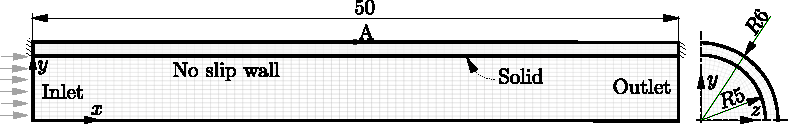
\includegraphics[scale=1]{figures/3dTube-geometry}
	\caption{Three-dimensional elastic tube: geometry and monitoring point A.}
	\label{fig:3dtube_geom}
\end{figure}

\paragraph{Purpose.}
A pressure pulse travelling through a fluid-filled elastic tube (Fig.~\ref{fig:3dtube_geom}) is the standard three-dimensional haemodynamic test of partitioned coupling under strong added mass ($\rho_s/\rho_f = 1.2$)~\citetodo{Formaggia et al.\ 2001; Gerbeau \& Vidrascu 2003; Fern\'andez \& Moubachir 2005}~\citep{kuttler2008fixed, Degroote2009}.
Most publications report only iteration counts and qualitative snapshots.

\paragraph{Problem.}
A quarter of the tube is modelled.
A $3\,\mathrm{ms}$ pressure pulse is applied at the inlet and the response is computed to $20\,\mathrm{ms}$, which includes the reflection from the outlet.
The fluid has $\rho_f = 1000\,\mathrm{kg/m^3}$, $\nu_f = 3\times10^{-6}\,\mathrm{m^2/s}$; the solid is Hookean linear elastic with small-strain kinematics (most published calculations use St Venant--Kirchhoff; the peak hoop strain is approximately $3\%$).

\paragraph{Reference.}
No tabulated values exist.
The available references are time histories at point A read from figures: \citet{Tukovic2018} (finite volume, BDF2, extracted exactly from vector graphics; same code lineage); and \citet{Lozovskiy2019} and \citet{Eken2016} (independent monolithic finite element codes, both using implicit Euler with $\Delta t = 10^{-4}\,\mathrm{s}$; raster-digitised to about $\pm3\times10^{-6}\,\mathrm{m}$).
The thick-wall long-wave estimate of the pulse-wave speed, $4.81\,\mathrm{m/s}$~\citep{Tukovic2018}, and the Moens--Korteweg speeds (5.2--5.7\,m/s) are approximate checks only.
The reference is therefore category C-weak.

\paragraph{Verification study.}
QoIs at point A are the maximum radial displacement $u_{r,\max}$ and its time, the incident trough of the axial displacement $u_{z,\min}$, the minimum radial displacement after reflection, the arrival time of the wavefront $t_\mathrm{arr}$ and the pulse-wave speed $c_p$.
The mesh study has two levels (16\,000 fluid/6\,400 solid cells and 128\,000/51\,200 cells, with $\Delta t$ halved); a third level (approximately $1.4\times10^6$ cells) is defined but has not been run.
The time-step study uses $\Delta t = 10^{-4}$ to $1.25\times10^{-5}\,\mathrm{s}$ on level 1.
A ``literature-discretisation'' run reproduces the implicit-Euler, $\Delta t = 10^{-4}\,\mathrm{s}$ set-up of the finite element references.
Robin--Neumann and IQN-ILS are compared on level 1.

\begin{table}[htbp]
	\centering
	\small
	\setlength{\tabcolsep}{5pt}
	\caption{3dTube: QoIs at point A on mesh levels 1 and 2 (BDF2, $\Delta t$ halved with the mesh), and the relative change between them.}
	\label{tab:3dtube}
	\begin{tabular}{lrrr}
		\toprule
		Quantity & Level 1 & Level 2 & Change \\
		\midrule
		$u_{r,\max}$ (mm) & 0.15984 & 0.15976 & $0.05\%$ \\
		$u_{z,\min}$ (mm) & $-0.08823$ & $-0.08660$ & $1.85\%$ \\
		$t_\mathrm{arr}$ (ms) & 5.874 & 5.854 & $0.34\%$ \\
		$c_p$ (m/s) & 4.771 & 4.695 & $1.58\%$ \\
		\bottomrule
	\end{tabular}
\end{table}

\paragraph{Findings.}
\begin{itemize}
	\item \emph{Time step.} Successive halvings of $\Delta t$ change $u_{r,\max}$ by $1.74\%$, $0.83\%$ and $0.016\%$, and $t_\mathrm{arr}$ by $2.23\%$, $0.44\%$ and $0.14\%$; the tutorial time step is converged to approximately $0.1\%$ in these QoIs.
	\item \emph{Mesh.} Between levels 1 and 2, $u_{r,\max}$ changes by only $0.05\%$, but $u_{z,\min}$ changes by $1.85\%$ and $c_p$ by $1.58\%$ (Table~\ref{tab:3dtube}). With two levels no order can be computed, and the axial displacement and wave speed are not yet shown to be converged.
	\item \emph{Literature discrepancy explained.} The published finite element peaks of $u_{r,\max}$ (approximately $0.119$ and $0.124\,\mathrm{mm}$) are some $21$--$24\%$ below the finite volume value of \citet{Tukovic2018} ($0.157\,\mathrm{mm}$). When the present code is run with the finite element discretisation in time (implicit Euler, $\Delta t = 10^{-4}\,\mathrm{s}$), its peaks lie within $+2.5\%$ of \citet{Lozovskiy2019} and $-1.4\%$ of \citet{Eken2016}. Most of the discrepancy between the finite element and finite volume literature is therefore explained by the numerical damping of the first-order, large-step time discretisation used in the published finite element calculations, not by the spatial discretisations or by the coupling.
	\item \emph{Converged comparison.} The level-2 BDF2 result, $u_{r,\max} = 0.15976\,\mathrm{mm}$, is $1.8\%$ above \citet{Tukovic2018}; $c_p = 4.695\,\mathrm{m/s}$ is $2.4\%$ below the approximate thick-wall estimate.
	\item \emph{Coupling.} Robin--Neumann and IQN-ILS histories differ by at most $0.27\%$ of the peak and the QoIs by at most $0.08\%$; Robin--Neumann needs 4.74 coupling iterations per step against 15.53 for IQN-ILS and is 4.1 times faster. The Robin--Neumann iteration count rises to 7.4 at the smallest time step; this has not been investigated.
\end{itemize}
% Derived: 0.1194/0.15694 - 1 = -23.9%; 0.1242/0.15694 - 1 = -20.9% (raster-digitised FE peaks vs Tukovic 2018 vector-extracted peak).

\todo{ESSENTIAL: run mesh level 3 (approximately $1.4\times10^6$ cells; estimated $>10$\,h on 6 ranks). Two levels do not support a convergence claim, and $u_{z,\min}$ still changes by $1.85\%$. COMSOL (or other independent code) solution with BDF2-type time integration at converged $\Delta t$ would add unique value: it would replace a same-lineage reference with an independent converged one and would test the time-discretisation explanation of the literature discrepancy from the finite element side.}

\paragraph{Role in the suite.}
This is the only three-dimensional transient case with mesh, time and coupling studies, and it yields a genuine ``benchmark revisited'' result: an apparent $\approx25\%$ disagreement between codes in the literature is largely a time-discretisation effect.
It also illustrates that a QoI-dependent conclusion is possible even with two mesh levels ($u_{r,\max}$ converged, $u_{z,\min}$ not).
Cost: level 1 425\,s and level 2 7\,197\,s on 4 ranks.
Limitations: two mesh levels; figure-digitised references; Hookean rather than St Venant--Kirchhoff solid; the pressure is ramped off over 3.0--3.1\,ms rather than instantaneously.

%%-------------------------------------------------------------------
\subsubsection{Modified lid-driven cavity}\label{sec:mok}
%%-------------------------------------------------------------------

\paragraph{Purpose.}
A lid-driven cavity with a flexible membrane bottom~\citetodo{Wall 1999 thesis; Mok 2001 thesis} is one of the oldest partitioned-coupling benchmarks~\citetodo{Gerbeau \& Vidrascu 2003}~\citep{kuttler2008fixed, Kassiotis2011}.
The membrane is tension-dominated (thickness $0.002\,\mathrm{m}$, $E = 250\,\mathrm{Pa}$) and undergoes large displacement (approximately $0.29\,\mathrm{m}$ in a $1\,\mathrm{m}$ cavity) under a periodically forced lid ($1-\cos(2\pi t/5)$); the cavity is nearly enclosed, with small openings that make the problem well posed for an incompressible fluid.

\paragraph{Reference: two inconsistent groups.}
The published midpoint histories fall into two mutually inconsistent groups (Fig.~\ref{fig:mok_refs}).
In group A (Mok, Wall, Gerbeau and Vidrascu) the openings are defined through the mesh and their size is not stated, so the problem depends on the mesh; the published peaks range from $0.177$ to $0.215\,\mathrm{m}$ and are not mutually consistent.
Group B (Vald\'es\citetodo{Vald\'es 2007 thesis}, the Kratos example\citetodo{Kratos Multiphysics example (Zorrilla)}, and Tiba et al.\citetodo{Tiba et al.\ 2026, arXiv:2609.16876 \emph{preprint}}) uses a fully specified inflow over a fixed $0.125\,\mathrm{m}$ opening and $p = 0$ at the outlet; within this group the peak displacement varies by $5.7\%$ and the oscillation amplitude by $20\%$.
\citet{Kassiotis2011} lies between the groups.
None of the published sources reports a mesh or time-step convergence study, and the Tiba et al.\ values are from a preprint and provide scalars only.
Two pilot runs show that the group-B definition reproduces group B, whereas traction-free conditions on both openings move the membrane downwards and reproduce neither group.
The reference is therefore category C-weak, and no single published value is treated as exact.

\begin{figure}[htbp]
	\centering
	% Source: solids4foam development, tutorials/fluidSolidInteraction/mokLidDrivenCavity/verification/reference/references_and_pilots.png (PR #497).
	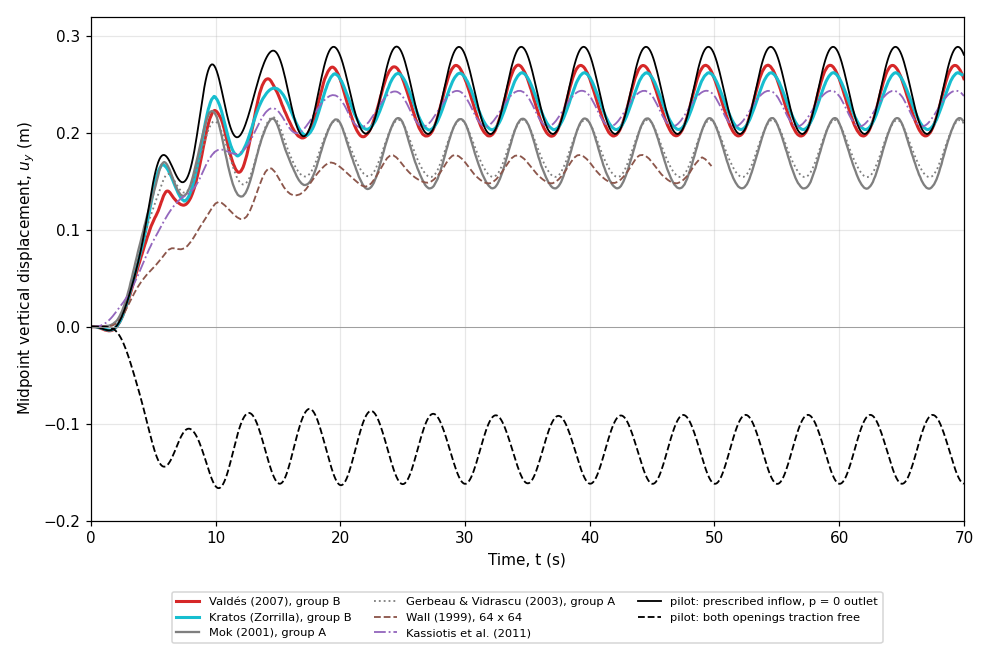
\includegraphics[width=0.85\textwidth]{figures/verification/mokLidDrivenCavity_references_and_pilots}
	\caption{Modified lid-driven cavity: published membrane-midpoint histories (group A: Mok, Wall, Gerbeau and Vidrascu; group B: Vald\'es, Kratos; Kassiotis et al.) and two pilot solids4foam runs ($32\times32$ mesh) with the group-B opening definition and with both openings traction free. Interim figure reproduced from the solids4foam verification output.}
	\label{fig:mok_refs}
\end{figure}
\todo{Replace Figure~\ref{fig:mok_refs} with a publication-quality figure that adds the converged ($96\times96$) solids4foam history and the group-B envelope, and drops the traction-free pilot or moves it to a separate panel. Confirm the extraction method and calibration of every curve before publication; the Kratos curve is raster-digitised (about $0.5\%$ of peak).}

\paragraph{Verification study.}
The QoIs are the mean peak, trough and time-mean of the membrane midpoint displacement over $t = 20$--$70\,\mathrm{s}$.
The mesh study uses $16^2$, $32^2$, $64^2$ and $96^2$ fluid cells with $\Delta t = 0.2$, $0.1$, $0.05$ and $0.025\,\mathrm{s}$; a $128^2$ run diverged (cause not isolated).
The time-step study uses $\Delta t = 0.1$, $0.05$ and $0.025\,\mathrm{s}$ on the $64^2$ mesh.
The standard solid (two or eight cells through the thickness) and the high-order solid are compared.

\begin{table}[htbp]
	\centering
	\small
	\setlength{\tabcolsep}{5pt}
	\caption{mokLidDrivenCavity: membrane-midpoint statistics (m) under combined mesh and time-step refinement, and the published group-B envelope. Group A peaks lie between 0.177 and 0.215\,m.}
	\label{tab:mok}
	\begin{tabular}{lrrr}
		\toprule
		Mesh ($\Delta t$) & Peak & Trough & Mean \\
		\midrule
		$16^2$ (0.2\,s) & 0.2934 & 0.1942 & 0.2426 \\
		$32^2$ (0.1\,s) & 0.2890 & 0.1986 & 0.2427 \\
		$64^2$ (0.05\,s) & 0.2870 & 0.2022 & 0.2437 \\
		$96^2$ (0.025\,s) & 0.2861 & 0.2044 & 0.2445 \\
		\midrule
		Group B envelope & 0.2619--0.2769 & 0.1967--0.2033 & 0.2316--0.2466 \\
		\bottomrule
	\end{tabular}
\end{table}

\paragraph{Findings.}
\begin{itemize}
	\item \emph{Self-convergence.} Successive changes in the peak are $1.56\%$, $1.26\%$ and $0.78\%$ of the peak; the observed order of the peak is approximately 1.2 (non-uniform final ratio), suggesting a limit near $0.285\,\mathrm{m}$, and that of the trough is below 0.5, leaving the trough uncertain by approximately $1$--$2\%$. The time step changes the response by $0.17\%$ and $0.04\%$ of the peak, so the error is dominated by the mesh.
	\item \emph{Comparison with the literature.} On the $96^2$ mesh the trough ($0.2044\,\mathrm{m}$) and the mean ($0.2445\,\mathrm{m}$) lie within or just outside the group-B envelope ($+0.56\%$ above the trough envelope), and the peak ($0.2861\,\mathrm{m}$) is $3.3\%$ above the largest group-B peak. Since the group-B sources are themselves single-mesh results that differ by $5.7\%$ in peak, this difference cannot be attributed to either side.
	\item \emph{Solid.} The standard and high-order solids agree to $0.04\%$: for a tension-dominated membrane the high-order solid gives no benefit (and costs 1.5 times more), in contrast to the bending-dominated collapsible channel (Section~\ref{sec:collapsible}).
	\item \emph{Coupling.} IQN-ILS needs 2.4--4.8 coupling iterations per step; Aitken relaxation needs approximately 9.9 and gives the same response (the difference has not been recorded quantitatively).
\end{itemize}

\paragraph{Role in the suite.}
The case is retained as an example of how a long-established benchmark can be ill defined: the literature contains two inconsistent problem definitions, neither supported by a convergence study.
The present results establish a self-converged solution for the fully specified group-B definition (to approximately $1\%$ in the peak, less well in the trough).
They are not a verification against an external reference.
\todo{An independent converged solution (COMSOL or another code) of the group-B definition, with its own mesh and time study, would add unique value and would make this a category-B case. Also: diagnose the $128^2$ divergence; Richardson estimates of peak and trough; quantify the IQN-ILS/Aitken difference.}


%%-------------------------------------------------------------------
\subsubsection{Flexible-bottom cavity [PROVISIONAL]}\label{sec:cavity}
%%-------------------------------------------------------------------

\todo{PROVISIONAL BENCHMARK: retain in main text only if (i) a clean partitioned mesh study with at least three levels in the asymptotic range is completed, including level 4 ($\Delta x = 0.0125$) at a reduced time step, together with a pseudo-time-step and coupling-tolerance check; and (ii) an independent converged reference (e.g.\ COMSOL, with its own mesh study) is obtained. The present reference is same-lineage and digitised (C-weak), and the steady displacement converges to a value approximately $5\%$ from it. All quasi-monolithic results for this case (simulationData/cavityFlexibleBottom, parent-paper Case~1) are deliberately NOT used as evidence. Otherwise move to supplementary material or drop.}

\begin{figure}[htbp]
	\centering
	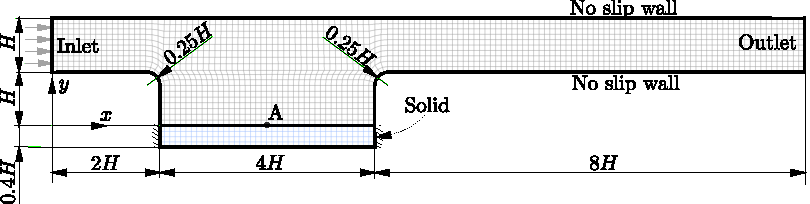
\includegraphics[scale=1]{figures/cavityFlexibleBottom-geometry}
	\caption{Channel flow over a cavity with a flexible bottom: geometry and boundary conditions.}
	\label{fig:cavity_geom_v}
\end{figure}

\paragraph{Why it could be valuable.}
Steady channel flow over a cavity with a flexible floor~\citep{Tukovic2018} (Fig.~\ref{fig:cavity_geom_v}), derived from a fluid benchmark~\citep{Juretic2010}, is the only steady internal-flow problem in the suite, and has large deformation of the floor ($u_y \approx -0.24\,\mathrm{m}$) at $Re = 100$.
It is inexpensive (about 10\,min serial for three levels).

\paragraph{Existing evidence.}
The reference is the mesh study of~\citet{Tukovic2018}, digitised from figures, computed with an earlier version of the same code family (category C-weak).
A partitioned (Aitken) mesh study with three levels ($\Delta x = 0.1$, $0.05$, $0.025\,\mathrm{m}$) gives steady displacements $u_y = -0.20246$, $-0.22883$ and $-0.23563\,\mathrm{m}$ at the monitoring point, i.e.\ $13.2\%$, $6.88\%$ and $5.59\%$ from the published values at the same spacing, with a net observed order of 1.96.
The interface force agrees with the published values to within $0.2\%$ on all three levels.
The displacement therefore converges at approximately second order, but towards a value about $5\%$ from the published curve, while the force agrees on every mesh.

\paragraph{Missing evidence.}
\begin{itemize}
	\item Level 4: diverges at the tutorial pseudo-time step ($\Delta t = 0.5\,\mathrm{s}$) with both Aitken and IQN-ILS, because the added-mass effect grows as interface cells shrink; it must be run with a smaller pseudo-time step.
	\item No coupling or tolerance study, and no partitioned pseudo-time-step study.
	\item The origin of the $5\%$ displacement offset at equal force is unexplained. Possible causes include a difference in solid model, material parameters, monitoring point or boundary conditions between the present set-up and that of~\citet{Tukovic2018}; an earlier solids4foam version gave $-0.219\,\mathrm{m}$ on the coarsest mesh, against $-0.20246\,\mathrm{m}$ now.
	\item An independent reference.
\end{itemize}

\paragraph{Promotion criterion.}
A clean partitioned three- to four-level study in the asymptotic range, an explanation of the displacement offset, and an independent converged COMSOL solution of the identical set-up.
If the independent solution agrees with the present converged displacement, the case would demonstrate that a same-lineage published curve was inaccurate; if it agrees with the published curve, it would expose a set-up or modelling difference.
Either outcome is informative, but neither can be claimed now.


%%%%%%%%%%%%%%%%%%%%%%%%%%%%%%%%%%%%%%%%%%%%%%%%%%%%%%%%%%%%%%%%%%
\subsection{Three-dimensional and realistic-complexity benchmarks}\label{sec:threeD}
%%%%%%%%%%%%%%%%%%%%%%%%%%%%%%%%%%%%%%%%%%%%%%%%%%%%%%%%%%%%%%%%%%

%%-------------------------------------------------------------------
\subsubsection{Beam in cross-flow [PROVISIONAL]}\label{sec:beam}
%%-------------------------------------------------------------------

\todo{PROVISIONAL BENCHMARK: retain in main text only if (i) a graded fluid-mesh family that resolves the near-body flow and boundary layer reaches the asymptotic range for both displacement and integrated force (three levels with consistent observed orders), with per-level values tabulated in CSV; and (ii) an independent converged reference is obtained, at least for the large-deformation (modified) form (COMSOL; or Gillebaart et al.\ 2016 if it tabulates the same configuration). Current uniform refinements are NOT asymptotic, and no convergence claim may be made from them.}

\begin{figure}[htbp]
	\centering
	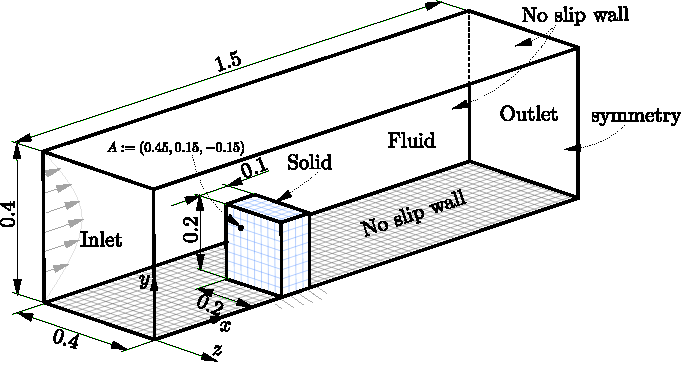
\includegraphics[scale=1]{figures/beamInCrossFlow-geometry}
	\caption{Beam in cross-flow: geometry (half domain with $z = 0$ symmetry) and monitoring point A.}
	\label{fig:beam_geom}
\end{figure}

\paragraph{Why it could be valuable.}
A thick elastic plate clamped in a three-dimensional channel flow (Fig.~\ref{fig:beam_geom}) is the only steady three-dimensional case in the suite, and the only three-dimensional large-deformation case.
Two forms share one geometry: an original small-deformation form ($E = 1.4\,\mathrm{MPa}$, $U_\mathrm{max} = 0.2\,\mathrm{m/s}$, $Re = 40$)~\citep{Richter2015} and a modified large-deformation form ($E = 10\,\mathrm{kPa}$, $U_\mathrm{max} = 0.3\,\mathrm{m/s}$)~\citep{Tukovic2018}, which together separate geometric nonlinearity from discretisation effects.

\paragraph{Existing evidence.}
\begin{itemize}
	\item \emph{References.} Original form: $u_x(A) = 5.95\times10^{-5}\,\mathrm{m}$ and $F_x = 1.33\,\mathrm{N}$ from an independent monolithic finite element code~\citep{Richter2015} (category C; which refinement level, and whether the values are extrapolated, remains to be checked). Modified form: values read from Fig.~28 of \citet{Tukovic2018}, a single unstructured mesh computed with an earlier version of the same code family (category C-weak).
	\item \emph{Mesh studies.} Uniform refinements by factors 1, 2, 4, 8 (original; finest approximately $7.6\times10^6$ cells, about 11\,h on 64 cores) and 1, 2, 3, 4, 8 (modified), with $\Delta t$ reduced with the mesh. On the finest original mesh, $u_x(A) = 5.95387\times10^{-5}\,\mathrm{m}$ ($+0.07\%$ from Richter) and $F_x = 1.310774\,\mathrm{N}$ ($-1.4\%$ from Richter). On the finest modified mesh the displacements differ from the same-lineage values by $-2.3\%$ ($u_x$), $-0.7\%$ ($u_y$) and $+2.3\%$ ($2u_z$).
	\item \emph{Non-asymptotic behaviour.} The final refinement still changes $u_x(A)$ by approximately $4.6\%$ (original) and $4.7\%$ (modified) (values read from the stored plots), and the transverse force $F_y$ (original) varies non-monotonically. The close agreement of the finest $u_x(A)$ with Richter therefore cannot be separated from coincidence.
	\item \emph{Displacement versus force.} On the finest original mesh $u_x(A)$ agrees with Richter to $0.07\%$ while $F_x$ differs by $1.4\%$, and the two converge differently under refinement. This is consistent with the integrated force being controlled by the resolution of the near-body velocity gradients, which uniform refinement of a coarse base mesh improves only slowly; it is a hypothesis to be tested by the graded-mesh study, not an established result.
	\item \emph{Coupling.} Robin--Neumann and IQN-ILS agree to within $0.4\%$ on the base mesh for both forms. The refined meshes were not re-run after a later change of the IQN-ILS default settings, which changed the base-mesh result by $0.01\%$.
\end{itemize}

\paragraph{Missing evidence and promotion criterion.}
\begin{itemize}
	\item A graded fluid-mesh family with boundary-layer resolution near the plate, reaching consistent three-level observed orders for $u_x(A)$, $u_y(A)$, $F_x$ and $F_y$, with Richardson estimates.
	\item Tabulated per-level values (currently only the finest values are tabulated; the others are read from plots).
	\item An independent time-step check (none exists; $\Delta t$ is scaled with the mesh).
	\item Confirmation of the Richter refinement level; an independent converged reference for the modified form (COMSOL, or Gillebaart et al.~\citep{Gillebaart2016} if applicable).
\end{itemize}

%%-------------------------------------------------------------------
\subsubsection{Hessenthaler three-dimensional benchmark [IN DEVELOPMENT]}\label{sec:hessenthaler}
%%-------------------------------------------------------------------

\todo{IN DEVELOPMENT --- placeholder only. No solids4foam case, verification driver or numerical result for this benchmark exists in the repository at the time of writing. Do not add numbers until the case and its verification study exist. Retain in the main text only if mesh, time-step and coupling-tolerance studies are completed with consistent observed orders for the principal QoIs.}

\paragraph{Intended role.}
The benchmark of Hessenthaler et al.\citetodo{Hessenthaler et al.\ 2017, IJNMBE, ``Experiment for validation of fluid--structure interaction models and algorithms''; check also the companion numerical paper} is intended as the realistic-complexity, fully three-dimensional capstone of the suite: a geometrically complex, three-dimensional, large-deformation FSI problem driven by periodic flow, at a cost that tests solver robustness and parallel performance rather than a single coupling mechanism.

\paragraph{Planned verification study.}
\begin{itemize}
	\item Problem definition and parameters taken from the published specification; deviations stated explicitly.
	\item QoIs to be defined (e.g.\ membrane/structure displacement at defined points, flow rate, pressure drop), with periodic-window statistics as in Section~\ref{sec:qoi}.
	\item Mesh study (at least three levels), time-step study (at least three levels) and a coupling-tolerance sweep, each with observed orders.
	\item An independent numerical reference, if available (COMSOL or published), classified according to Table~\ref{tab:ref_hierarchy}.
\end{itemize}

\paragraph{Experimental data.}
The benchmark is accompanied by phase-contrast MRI and other experimental measurements.
These are \emph{validation} data: agreement with them depends on the mathematical model as well as on the numerics, and they are not used as evidence of numerical verification in this paper.
If included, they will be presented separately, as context, after the numerical verification.


%%%%%%%%%%%%%%%%%%%%%%%%%%%%%%%%%%%%%%%%%%%%%%%%%%%%%%%%%%%%%%%%%%
\subsection{Additional transient benchmark}\label{sec:additional}
%%%%%%%%%%%%%%%%%%%%%%%%%%%%%%%%%%%%%%%%%%%%%%%%%%%%%%%%%%%%%%%%%%

%%-------------------------------------------------------------------
\subsubsection{Blob in treacle [PROVISIONAL]}\label{sec:blob}
%%-------------------------------------------------------------------

\todo{PROVISIONAL BENCHMARK / possible supplementary material: retain in the main text only if (i) an independent converged reference (COMSOL being arranged) replaces the coarse, figure-digitised preprint reference; and (ii) the time study is extended below $\Delta t = 0.03125\,\mathrm{s}$ with tightened coupling and solver tolerances, showing orders close to 2 rather than the present super-nominal 2.4--2.5. Otherwise move to supplementary material.}

\begin{figure}[htbp]
	\centering
	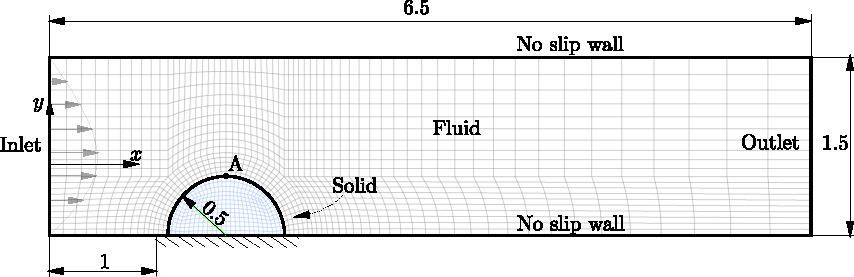
\includegraphics[scale=1]{figures/blobInTreacle-geometry}
	\caption{Blob in treacle: elastic half-cylinder in a viscous channel flow; geometry and monitoring (top) point.}
	\label{fig:blob_geom}
\end{figure}

\paragraph{Why it could be valuable.}
An elastic half-cylinder in a highly viscous channel flow (Fig.~\ref{fig:blob_geom}; $\rho_f = 1$, $\nu_f = 1$, ramped to a steady state at $t = 2\,\mathrm{s}$), proposed by~\citet{Liu2014} to measure the temporal order of a coupled scheme, is a strongly damped, large-deformation problem (top-point $u_x \approx 0.12\,\mathrm{m}$ for a $0.1\,\mathrm{m}$ radius) in which the temporal error can be isolated cleanly.

\paragraph{Existing evidence.}
\begin{itemize}
	\item \emph{Reference (C-weak).} \citet{Liu2014} report only self-convergence norms. The preprint version\citetodo{Liu et al., arXiv:1401.0082} gives interface shapes at $t = 1\,\mathrm{s}$ (P5/P4/P5 elements, first-order time integration with $\Delta t = 0.025\,\mathrm{s}$, with an estimated time error of approximately $4\%$ of its own) and at steady state (a coarse mesh of 1\,239 fluid and 370 solid triangles); these were vector-extracted from figures.
	\item \emph{Time step.} At $t = 1\,\mathrm{s}$, $\Delta t = 0.25$, $0.125$, $0.0625$, $0.03125\,\mathrm{s}$ give top-point $u_x = 0.0558737$, $0.0564184$, $0.0565219$ and $0.0565398\,\mathrm{m}$, with observed orders 2.39 and 2.54 ($u_x$) and 2.39 and 2.41 (interface shape). Below $\Delta t = 0.03125\,\mathrm{s}$ the changes reach the coupling/solver-tolerance level (approximately $10^{-5}\,\mathrm{m}$). Orders above the formal value of 2 indicate that this large-$\Delta t$ sequence is not yet in the asymptotic range; the evidence supports ``at least second-order'' behaviour over this range, not a measured order of 2.
	\item \emph{Mesh.} Four levels (factors 0.5--4) give steady $u_x = 0.108206$, $0.117301$, $0.119698$, $0.120152\,\mathrm{m}$, with an observed order of 2.40 and a Richardson estimate of $0.12026\,\mathrm{m}$; the finest level is within $0.1\%$ of it.
	\item \emph{Comparison.} At $t = 1\,\mathrm{s}$ the interface shape is within $1.6\%$ of the preprint, inside its own approximately $4\%$ time error. At steady state, $u_x$ is $7.4\%$ smaller than the preprint value and $|u_y|$ $20\%$ larger; this offset is attributed to the coarseness of the reference mesh, but this attribution is unconfirmed.
	\item \emph{Coupling.} No coupling comparison or tolerance study exists; the finest mesh requires $\Delta t = 0.005\,\mathrm{s}$ because of IQN-ILS stagnation.
\end{itemize}

\paragraph{Promotion criterion.}
An independent converged reference at $t = 1\,\mathrm{s}$ and at steady state; a time study extended to smaller $\Delta t$ with tightened tolerances; a coupling-tolerance check.
The case's distinctive contribution, a clean temporal-order measurement in a viscous large-deformation problem, partly overlaps with ringAddedMass and collapsibleChannel, which is why it may ultimately be moved to supplementary material.

%%%%%%%%%%%%%%%%%%%%%%%%%%%%%%%%%%%%%%%%%%%%%%%%%%%%%%%%%%%%%%%%%%
\section{Cross-benchmark analysis}\label{sec:cross_benchmark}
%%%%%%%%%%%%%%%%%%%%%%%%%%%%%%%%%%%%%%%%%%%%%%%%%%%%%%%%%%%%%%%%%%
% Synthesis of Section 5. All values are repeated from Section 5 / the
% evidence inventory / paper-data evidence reports, except the Hessenthaler
% convergence-test evidence (Section iterative_errors), which has no Section-5
% counterpart because that case has no convergence results yet.

\todo{Synthesis based on the evidence available on 2026-10-10. Conclusions will change when: (a) the beamInCrossFlow (Richter) and Hessenthaler verification campaigns are completed; (b) independent references become available (3dTube, mokLidDrivenCavity first); (c) the Hron--Turek geometric-singularity hypothesis is tested.}

This section draws together the findings of Section~\ref{sec:benchmark_suite} by theme.
In this suite the strength of a verification statement is usually limited by the quality of the reference, the number of refinement levels that could be afforded, or the iterative error, or by sub-nominal convergence whose cause is only partly identified.
Verification also exposed defects that agreement with a reference would not have shown: an $O(\Delta t)$ boundary-flux inconsistency (womersleyTube), a compiler-dependent aliasing error and a mesh-dependent interpolation degeneracy (3dTube), and a coupling convergence test that can accept unconverged steps (Hessenthaler); these are collected in Section~\ref{sec:defects}.
The observations are specific to this suite and to one code family, and are not offered as universal.

%%%%%%%%%%%%%%%%%%%%%%%%%%%%%%%%%%%%%%%%%%%%%%%%%%%%%%%%%%%%%%%%%%
\subsection{Nominal and observed convergence}\label{sec:cross_convergence}
%%%%%%%%%%%%%%%%%%%%%%%%%%%%%%%%%%%%%%%%%%%%%%%%%%%%%%%%%%%%%%%%%%

\begin{table}[htbp]
	\centering
	\footnotesize
	\setlength{\tabcolsep}{3pt}
	\caption{Observed orders across the suite (formal order 2 in space and time). ``SD'': successive differences of three or more levels (reference-free); ``vs exact'': error against an exact reference; ``2-level vs ref.'': apparent order from two levels against a non-exact reference; ``scaled'': $\Delta t$ reduced with $h$.}
	\label{tab:orders}
	\begin{tabular}{p{3.0cm}p{4.6cm}p{3.4cm}p{2.8cm}}
		\toprule
		Case & Space & Time & Basis \\
		\midrule
		ringAddedMass & freq.\ converged on coarsest mesh; ratio 1.68--1.77; standard solid 1.66 & 1.90--2.14 & vs exact; Richardson \\
		womersleyTube & 2.01--2.05 (amplitudes, profile, speed); 1.92 (flow phase); 1.40 (wall phase); attenuation at linear-theory level & 1.86--2.14 (1.29--1.84 before end-flux fix) & SD; errors vs exact \\
		collapsibleChannel & 1.7, 2.4, then reference floor & 1.8, 2.0 & vs ref.\ (B); SD (time) \\
		Hron--Turek FSI1 & 1.5--1.7 & -- & 2-level vs ref.\ (B) \\
		Hron--Turek FSI3 & displacements 0.9--1.1; drag amplitude 0.74 (scaled) & $\leq1.7\%$ change (2x, $\Delta t$ and tolerance) & SD \\
		3dTube & $u_{z,\min}$ 0.87, $t_\mathrm{arr}$ 0.72; $u_{r,\max}$ not defined (changes grow) & 0.1--0.2\% change at the fine-level $\Delta t$ & SD \\
		mokLidDrivenCavity & peak $\approx1.2$; trough $<0.5$ (scaled) & changes $0.17$, $0.04\%$ & SD \\
		cavityFlexibleBottom$^\ast$ & 1.96 ($u_y$; one triple, level 4 diverged) & -- & SD \\
		beamInCrossFlow$^\ast$ & in progress & -- & -- \\
		blobInTreacle$^\ast$ & 2.40 (super-nominal) & 2.39--2.54 (super-nominal) & SD \\
		\bottomrule
		\multicolumn{4}{l}{$^\ast$ Provisional cases.}
	\end{tabular}
\end{table}

Table~\ref{tab:orders} collects the observed orders, from which three observations follow.

\emph{Observed orders can depart from the nominal order.}
Among the category-A cases, ringAddedMass exhibits near-second-order temporal convergence, while the amplitude-type womersleyTube quantities exhibit near-second-order spatial convergence.
Independently of reference quality, collapsibleChannel also shows near-second-order behaviour, in space against its category-B reference (orders 1.7 and 2.4 before the reference floor) and in time by self-convergence (1.8 and 2.0).
womersleyTube first showed temporal orders of 1.3--1.8 that fell towards one as $\Delta t$ was refined, on every mesh.
The orders are reference-free observations, but the diagnosis relied on the exact reference and on fluid-only and end-flux diagnostics: the deficit came from an $O(\Delta t)$ mass-flux inconsistency at the artificial tube ends, where the exact pressure and velocity gradient are imposed, not from the coupling (Section~\ref{sec:womersley}).
With a flux-consistent end treatment every QoI converges at second order in time over the steps used (formally, an $O(\Delta t\,h)$ boundary term remains, as for standard fixed-pressure outlets), and the finest solutions lie within $0.12\%$ of the continuum solution ($0.2\%$ for the attenuation, at the linear-theory level).
In ringAddedMass, by contrast, the exact reference allows the remaining $-0.13\%$ frequency error at a practical resolution to be attributed to the BDF2 phase error.

\emph{Two levels do not establish convergence, and super-nominal orders are a warning.}
Third levels changed the conclusions drawn from two in both cases where they were added.
In Hron--Turek FSI3 the two-level apparent orders of 2.6--3.8 arose from a sequence crossing the reference value, and the three-level observed order of the displacements is about one.
In 3dTube the small two-level change in $u_{r,\max}$ reported earlier was obtained with an interface interpolation operator that changed between the levels; after correction its changes grow on the third level.
FSI1 and FSI2 still have two levels, so the most widely used benchmarks in the suite remain the least completely verified.
Orders well above the formal value (the FSI3 filtered lift amplitude, 3.1; the rigid-flag force amplitudes, 2.8--3.3; the blobInTreacle temporal orders, 2.4--2.5) are interpreted as pre-asymptotic; no super-convergence is claimed, and they are not used for extrapolation.

\emph{Coupled limit-cycle QoIs can converge sub-nominally when the components behave well.}
In Hron--Turek FSI3 the solid alone approaches second order, the rigid-flag fluid converges to within the reference uncertainty, and the code defects of 3dTube have no effect; yet the coupled displacements converge at an observed order of about one, and the in-phase fluid force under the replayed coupled motion shows the same behaviour under every valid fluid treatment tested (Section~\ref{sec:fsi23}).
A self-excited amplitude is set by a balance of small differences between large loads, so a sub-nominal order in the in-phase load can appear as a sub-nominal order in the amplitude.
Two statements must therefore be kept apart: ``our result disagrees with the reference'' and ``our result is not yet resolved''.
At 4x the FSI3 displacements differ from Featflow by more than the reference's level-to-level change, but they are still changing at first order; neither the code nor the reference is shown to be wrong by this comparison.

\emph{Combined space--time refinement conceals the balance of errors.}
Where space and time have been separated, the balance differs strongly: in 3dTube the temporal error at the fine-level $\Delta t$ ($0.1$--$0.2\%$) is several times smaller than the level-2-to-3 change ($0.3$--$1.0\%$), in mokLidDrivenCavity it is an order of magnitude below the spatial error, in ringAddedMass it dominates the frequency, and in womersleyTube, once the end-flux inconsistency is removed, it is a tenth or less of the finest-mesh error for most QoIs (before, the two were similar).
Scaled studies cannot show which dominates unless supplemented, as for Hron--Turek FSI3 and 3dTube, by time-step checks on the finer levels.

%%%%%%%%%%%%%%%%%%%%%%%%%%%%%%%%%%%%%%%%%%%%%%%%%%%%%%%%%%%%%%%%%%
\subsection{Dependence on the quantity of interest}\label{sec:qoi_dependence}
%%%%%%%%%%%%%%%%%%%%%%%%%%%%%%%%%%%%%%%%%%%%%%%%%%%%%%%%%%%%%%%%%%

In every case with more than one QoI, the QoIs converge at substantially different rates (Table~\ref{tab:qoi_dependence}), so a verification statement made on one QoI says little about the others.

\begin{table}[htbp]
	\centering
	\footnotesize
	\setlength{\tabcolsep}{3pt}
	\caption{Faster- and slower-converging QoIs within each case (finest available level).}
	\label{tab:qoi_dependence}
	\begin{tabular}{p{2.8cm}p{5.4cm}p{5.4cm}}
		\toprule
		Case & Faster & Slower \\
		\midrule
		womersleyTube & flow-rate, wall amplitude, wave speed: order $\approx2$, error $\leq0.04\%$ & wall phase (order 1.40); attenuation (error $-0.2\%$, at the linear-theory level) \\
		Hron--Turek FSI1 (2x) & drag $0.24\%$ & $u_y$ $4.64\%$ \\
		Hron--Turek FSI3 (4x) & drag mean and frequency: within $0.3\%$ of the reference & displacements: order $\approx1$; force amplitudes $7.6$--$10.4\%$ above the reference, not asymptotic \\
		Hron--Turek FSI2 (2x) & drag mean $0.5\%$; $u_y$ amplitude $1.3\%$ & lift amplitude $7.8\%$, not converging \\
		3dTube & $u_{z,\min}$, $t_\mathrm{arr}$: monotone, orders 0.87, 0.72 & $u_{r,\max}$, $c_p$: changes grow ($u_{r,\max}$ $0.20\%$, $0.60\%$) \\
		mokLidDrivenCavity & peak (order $\approx1.2$) & trough (order $<0.5$) \\
		cavityFlexibleBottom$^\ast$ & $F_y$: within $0.2\%$ on all levels & $u_y$: 13.2\% $\to$ 5.6\% \\
				\bottomrule
	\end{tabular}
\end{table}

The pattern is not simply that displacements converge faster than forces.
Time-mean integrated forces (Hron--Turek drag, cavityFlexibleBottom vertical force) are often the \emph{fastest}-converging quantities, plausibly because they are dominated by a global pressure balance.
The slowest are of three kinds:
(i) oscillation amplitudes of forces that result from near-cancellation of larger contributions, above all the Hron--Turek lift amplitude, which is also the QoI most sensitive to the coupling tolerance;
(ii) phase- and attenuation-type quantities, or small components, such as the Womersley wall phase and attenuation ($\mathrm{Im}(k)$ is 14\% of $\mathrm{Re}(k)$) and the transverse tip displacement of FSI1; and
(iii) loads that set a self-excited response, such as the in-phase fluid force on the Hron--Turek flag, which converges at an observed order of about one under a fixed motion although the force amplitude converges quickly.
A benchmark should therefore report several QoI types (a displacement, a mean force, an oscillatory force amplitude or phase, and a frequency where applicable), and the slowest QoI on which a claim is made determines the resolution required.

%%%%%%%%%%%%%%%%%%%%%%%%%%%%%%%%%%%%%%%%%%%%%%%%%%%%%%%%%%%%%%%%%%
\subsection{Iterative and coupling errors}\label{sec:iterative_errors}
%%%%%%%%%%%%%%%%%%%%%%%%%%%%%%%%%%%%%%%%%%%%%%%%%%%%%%%%%%%%%%%%%%

The iterative error is the least systematically quantified component of the error budget in the present suite.

\emph{Direct tolerance evidence is limited.}
Hron--Turek FSI2 contains a coupling-tolerance sweep, and it shows that a tolerance of $10^{-5}$ inflates the lift amplitude by $13\%$ (1x) and $30\%$ (2x): the effect grows with refinement, so a tolerance chosen on a coarse mesh can contaminate a fine-mesh result.
FSI3 shows the same mechanism in time: at a fixed tolerance of $10^{-5}$ the step-to-step force noise grows as $\Delta t$ falls (lift $7.3\,\mathrm{N/m}$ rms at the 4x step against $1.7\,\mathrm{N/m}$ at the 2x step), inflating extrema-based force amplitudes while leaving the displacements unaffected, and at the finest step IQN-ILS stalls above a tolerance of $10^{-6}$.
Elsewhere, the iterative error is bounded only indirectly.

\emph{A converged-looking QoI can carry an accumulated coupling error.}
In the Hessenthaler verification campaign (Section~\ref{sec:hessenthaler}; OpenFOAM-v2412, IQN-ILS, tolerance $10^{-4}$, $\Delta t = 0.002\,\mathrm{s}$, 40\,000 steps to $t = 80\,\mathrm{s}$), the legacy test $\min(r_1, r_2)$ of Eq.~\eqref{eq:coupling_residuals} accepted steps after about three iterations once the flow had become quasi-steady, because $r_2$, normalised by the total tip deflection of $\approx17\,\mathrm{mm}$, was small (median $3.5\times10^{-5}$) whatever the reduction within the step.
After $t = 1\,\mathrm{s}$ every step was accepted with $r_1 > 10^{-4}$ (median $\approx6.8\times10^{-2}$; $87$--$91\%$ of steps with $r_1 > 10^{-2}$), the fluid interface lagged the solid by $\approx0.03\,\mathrm{mm}$, and the flap tip crept upwards at $+0.003$--$0.005\,\mathrm{mm/s}$ ($16.84$, $16.90$ and $16.98\,\mathrm{mm}$ at $t = 30$, $60$ and $80\,\mathrm{s}$), by more than the spatial differences under study.
Neither the fluid nor the solid alone drifted.
Restarted from the $80\,\mathrm{s}$ state with the strict test $\max(r_1, r_2)$ (10--11 iterations per step), the tip settled within $\approx0.3\,\mathrm{s}$ to a plateau of $17.0195\,\mathrm{mm}$, flat to $\pm0.0002\,\mathrm{mm}$ over $7.5\,\mathrm{s}$.
Strict restarts from different default-test states did not return to one value ($17.02$ and $16.90\,\mathrm{mm}$), so the accumulated error leaves history in the solution, and a clean reference requires the strict test from $t = 0$ (solids4foam issue \#552).
A steadiness check on the QoI --- for example a change below $0.04\%$ over the last second --- would have accepted the drifting solution.
The lesson is general to partitioned codes: a convergence measure normalised by a large total quantity can be met without converging the step, and the error it admits is invisible to checks on the solution itself; the residual reduction at acceptance should be reported.

\todo{The Hessenthaler numbers above were obtained on a tree without solids4foam PR \#546; the finding concerns the convergence test and is not expected to depend on it, but confirm with the A/B check. Evidence: solids4foam branch verification/hessenthaler-phaseI, commit 9f33c42a2, \texttt{hessenthalerFsi/verification/README.md}; solids4foam issue \#552.}

\emph{Iterative floors can limit refinement studies.}
In collapsibleChannel the IQN-ILS/Robin--Neumann difference does not decrease with refinement and, at the finest fluid mesh, is comparable with the remaining discretisation error and the reference uncertainty; in blobInTreacle the time study cannot be continued below $\Delta t = 0.03125\,\mathrm{s}$ because the changes reach the tolerance level.
In both, the iterative error rather than the discretisation bounds what can be verified.

\emph{Internal agreement is not external verification.}
IQN-ILS and Robin--Neumann agree to $0.03\%$ (ringAddedMass frequency), $2.2\times10^{-4}$ (womersleyTube), $0.01\%$ (FSI1), and $0.07\%$ (3dTube QoIs).
This bounds the iterative error relative to these differences and checks the implementations against each other; it says nothing about the shared discretisation error, nor about whether the common limit is the continuum solution.
FSI3 shows that the two need not agree to the coupling tolerance when the Robin--Neumann scheme modifies the discrete interface condition.

\emph{Coupling algorithms can affect solution quality as well as cost.}
In ringAddedMass, IQN-ILS produces a mesh-dependent amplitude loss that Robin--Neumann does not (mechanism unknown); and the cheaper algorithm is case dependent (IQN-ILS in ringAddedMass and FSI3, Robin--Neumann in womersleyTube and 3dTube).

\todo{ESSENTIAL: one or two representative coupling-tolerance sweeps (at least two decades, strict test) at fixed discretisation, e.g.\ ringAddedMass (strong level) and collapsibleChannel, so that the claim ``iterative error $\ll$ discretisation error'' rests on more than the Hron--Turek cases; and the $r_1$-at-acceptance audit of Section~\ref{sec:convergence_method}.}

%%%%%%%%%%%%%%%%%%%%%%%%%%%%%%%%%%%%%%%%%%%%%%%%%%%%%%%%%%%%%%%%%%
\subsection{Defects exposed by verification}\label{sec:defects}
%%%%%%%%%%%%%%%%%%%%%%%%%%%%%%%%%%%%%%%%%%%%%%%%%%%%%%%%%%%%%%%%%%

Four defects or hazards in the code under test were found by the studies of Section~\ref{sec:benchmark_suite}, none by comparison with a published value (Table~\ref{tab:defects}).

\begin{table}[htbp]
	\centering
	\footnotesize
	\setlength{\tabcolsep}{3pt}
	\caption{Defects and hazards exposed by verification, and how they were found.}
	\label{tab:defects}
	\begin{tabular}{p{2.6cm}p{5.6cm}p{5.6cm}}
		\toprule
		Case & Defect & How it was found \\
		\midrule
		womersleyTube & $O(\Delta t)$ inconsistency of the end flux under a mixed velocity condition & temporal order falling towards one against an exact reference \\
		3dTube & wall viscous force miscompiled at \texttt{-O3} (temporary-storage aliasing under \texttt{\_\_restrict\_\_}) & deterministic $1.5$--$3\%$ difference in one QoI between two platforms \\
		3dTube & degenerate barycentric weights below a fixed absolute area threshold; interpolation operator changed with mesh level & first divergence after the fix above; broken symmetry and rank dependence \\
		Hessenthaler & legacy coupling test $\min(r_1, r_2)$ accepts unconverged steps in quasi-steady phases & slow drift larger than the spatial differences; residuals at acceptance \\
		\bottomrule
	\end{tabular}
\end{table}

Two observations follow.
First, the toolchain belongs in the verification matrix.
The 3dTube aliasing defect produced a reproducible difference between two platforms that looked like a platform or round-off effect, and a study on one platform, at any resolution, would have reported either the correct or the incorrect result without warning.
Its root cause lies in the reuse of temporary storage by OpenFOAM's field products combined with \texttt{\_\_restrict\_\_}, so it is not specific to solids4foam; the audit for the fix found about 15 further sites of the same mechanism in solids4foam.
Second, a defect can switch on with refinement: the barycentric degeneracy affected levels 2 and 3 of 3dTube but not level 1, so the mesh study compared different interpolation operators, and its apparent convergence of the peak displacement was not evidence about the discretisation.
Cross-platform replication, decomposition invariance and symmetry checks are inexpensive and were decisive; they should accompany refinement studies of coupled codes.

%%%%%%%%%%%%%%%%%%%%%%%%%%%%%%%%%%%%%%%%%%%%%%%%%%%%%%%%%%%%%%%%%%
\subsection{Reliability of published benchmark values}\label{sec:published_reliability}
%%%%%%%%%%%%%%%%%%%%%%%%%%%%%%%%%%%%%%%%%%%%%%%%%%%%%%%%%%%%%%%%%%

Among the literature-referenced problems in the suite, only the Featflow FSI1 table and the regenerated collapsible-channel reference are both independent and accompanied by convergence evidence at the resolution used here (Table~\ref{tab:published}).
This is a statement about the specific values used, not about the quality of the FSI benchmark literature in general.

\begin{table}[htbp]
	\centering
	\footnotesize
	\setlength{\tabcolsep}{3pt}
	\caption{Issues found with published benchmark values.}
	\label{tab:published}
	\begin{tabular}{p{2.8cm}p{5.8cm}p{5.0cm}}
		\toprule
		Case & Issue & Consequence \\
		\midrule
		Hron--Turek FSI2/3 & Summary values of~\citet{Turek2006} differ from Featflow tables (FSI3 drag amplitude $-18\%$; rounded frequencies); Featflow level 3$\to$4 changes 1.6--4.5\% (FSI3 displacements and force amplitudes), 0.9--2.5\% (FSI2) & Choice of source changes conclusions; FSI3 reference uncertain by 3--5\% in $u_x$ and force amplitudes \\
		3dTube & Independent references use implicit Euler, $\Delta t = 10^{-4}\,\mathrm{s}$, without time-step studies; peaks 20--25\% below BDF2 values; figure-digitised & Implicit Euler in the present code reproduces 92--115\% of the gap \\
		mokLidDrivenCavity & Two inconsistent problem definitions; mesh-dependent openings; no convincing convergence studies; group-B spread 5.7\% (peak) & No published value can be treated as correct \\
		collapsibleChannel & Published problem (pre-stressed, massless wall) unsuitable for continuum/partitioned comparison & Modified problem and regenerated reference used \\
		beamInCrossFlow & Quoted values ($5.95\times10^{-5}\,\mathrm{m}$, $1.33\,\mathrm{N}$) are rounded extrapolations of \citet{Richter2012}, often cited to a later paper; earlier calculations solved a different beam position, monitoring point and inflow & Comparison withdrawn; campaign rebuilt to the published definition \\
		cavityFlexibleBottom & Same-lineage, digitised & Offset of $\sim5\%$ unexplained \\
		blobInTreacle & Preprint figures only; first-order time, coarse steady mesh & Steady offset of 7--20\% unexplained \\
		\bottomrule
	\end{tabular}
\end{table}

The table illustrates the central distinction of Section~\ref{sec:verification_methodology}: a widely used benchmark problem does not automatically provide a trustworthy benchmark solution.
The same problem can carry several published ``reference values'', and an $18\%$ difference in a quoted force amplitude exceeds the 2x-to-4x change of every FSI3 quantity.
Disagreements between codes can originate in the discretisation of the reference rather than of the code under test (3dTube), so a discrepancy with a published curve should not be resolved by tuning the code; and same-lineage references, though useful for regression and for diagnosing set-up differences, cannot expose common-mode errors.

%%%%%%%%%%%%%%%%%%%%%%%%%%%%%%%%%%%%%%%%%%%%%%%%%%%%%%%%%%%%%%%%%%
\subsection{Cost and dimensionality}\label{sec:cost}
%%%%%%%%%%%%%%%%%%%%%%%%%%%%%%%%%%%%%%%%%%%%%%%%%%%%%%%%%%%%%%%%%%

\begin{table}[htbp]
	\centering
	\footnotesize
	\setlength{\tabcolsep}{3pt}
	\caption{Recorded computational cost of the verification studies. Hardware and core counts differ between cases, so the figures indicate orders of magnitude only.}
	\label{tab:cost}
	\begin{tabular}{p{3.0cm}p{10.8cm}}
		\toprule
		Case & Recorded cost \\
		\midrule
		ringAddedMass & tutorial $\approx75$\,s serial; full study (35 runs) $\approx30$\,min with 32 concurrent serial runs \\
		womersleyTube & runs 2.5--25\,min serial; full study $\approx30$\,min on 5 cores \\
		collapsibleChannel & tutorial $\approx10$\,min; finest fluid mesh 70\,min; full sweep $\approx2.5$\,h (one case per core); serial only \\
		Hron--Turek FSI1 & 1x 781\,s serial; 2x 3\,062\,s on 2 ranks; 4x estimated $>14$\,h on 3 ranks \\
		Hron--Turek FSI3 & 1x 1.4\,h serial; 2x 5.5\,h on 8 ranks; 4x 40.8\,h on 32 ranks (no speed-up beyond 32 ranks); OpenFOAM-v2512 \\
		Hron--Turek FSI2 & 1x 1.1--1.2\,h serial; 2x 4.0--4.1\,h on 7--8 ranks \\
		3dTube & level 1 504\,s on 4 ranks; level 2 3\,641\,s on 8 ranks; level 3 22\,502\,s (6.25\,h) on 32 ranks ($\approx720$ core-hours) \\
		mokLidDrivenCavity & $96^2$ 3\,729\,s on 2 ranks; quick run $\approx7$\,min \\
		cavityFlexibleBottom$^\ast$ & three-level sweep $\approx10$\,min serial \\
		beamInCrossFlow$^\ast$ & in progress \\
		blobInTreacle$^\ast$ & full study $\approx33$\,min \\
		\bottomrule
	\end{tabular}
\end{table}

Cost rises by roughly four orders of magnitude from the exact-reference problems to the finest three-dimensional calculations (Table~\ref{tab:cost}), and the completeness of the evidence falls in the opposite direction: the inexpensive two-dimensional and axisymmetric problems have three or more levels in space and time and exact or independent references, whereas the three-dimensional problems have three levels with sub-nominal or undefined orders (3dTube) or, so far, no completed study (beamInCrossFlow, Hessenthaler). Even in two dimensions a third level can cost an order of magnitude more than the second (Hron--Turek FSI3: 40.8\,h on 32 ranks at 4x, without further strong scaling).
This illustrates one practical reason why rigorous convergence evidence becomes scarcer as geometric and computational complexity increase, and it motivates a tiered suite (Section~\ref{sec:recommended_suite}).
Which error source dominates is case dependent: in the thin-walled two-dimensional collapsibleChannel the solid discretisation can dominate ($17.4\%$ versus $0.44\%$ for linear versus cubic solid), whereas in Hron--Turek FSI3 refining the solid alone accounts for only $\approx5\%$ of the change in the $u_y$ amplitude.
\todo{Revisit once the beamInCrossFlow and Hessenthaler campaigns are complete; add cost per degree of freedom and per time step if comparable hardware is used.}

%%%%%%%%%%%%%%%%%%%%%%%%%%%%%%%%%%%%%%%%%%%%%%%%%%%%%%%%%%%%%%%%%%
\section{Recommended verification suite}\label{sec:recommended_suite}
%%%%%%%%%%%%%%%%%%%%%%%%%%%%%%%%%%%%%%%%%%%%%%%%%%%%%%%%%%%%%%%%%%

\todo{WORKING PROPOSAL. Final membership is not frozen; decisions marked below depend on outstanding evidence (paper-data/manuscript\_todos.md).}

Sections~\ref{sec:benchmark_suite} and~\ref{sec:cross_benchmark} suggest that no single benchmark verifies a continuum FSI code, and that the most widely used benchmarks are not the most discriminating.
We therefore propose a tiered suite.
The core suite is inexpensive enough to be run routinely, for example before each release or after a change to a discretisation or coupling algorithm, and is built around problems with exact or independently converged references.
The extended suite contains three-dimensional, geometrically complex or expensive problems that test behaviour under more realistic conditions and are run less often.

%%%%%%%%%%%%%%%%%%%%%%%%%%%%%%%%%%%%%%%%%%%%%%%%%%%%%%%%%%%%%%%%%%
\subsection{Core suite}\label{sec:core_suite}
%%%%%%%%%%%%%%%%%%%%%%%%%%%%%%%%%%%%%%%%%%%%%%%%%%%%%%%%%%%%%%%%%%

\begin{table}[htbp]
	\centering
	\footnotesize
	\setlength{\tabcolsep}{3pt}
	\caption{Proposed core suite (working proposal).}
	\label{tab:core_suite}
	\begin{tabular}{p{2.8cm}p{1.0cm}p{6.4cm}p{3.4cm}}
		\toprule
		Case & Ref. & What it verifies & Status \\
		\midrule
		ringAddedMass & A & added-mass coupling over $\mu = 0.1$--$10$; temporal order; solid-independent check via wet/dry ratio & core \\
		womersleyTube & A & viscous wave propagation; amplitude and phase; temporal order & core; open time-order finding \\
		collapsibleChannel & B & large-deformation bending wall; strong added mass; solid discretisation; partitioned robustness & core (serial; $\approx2.5$\,h full sweep) \\
		Hron--Turek FSI1 & B & steady large-deformation coupling & core; third level desirable \\
		mokLidDrivenCavity & C-weak & self-convergence of a tension-dominated membrane; definition sensitivity & core candidate; see note \\
		\bottomrule
	\end{tabular}
\end{table}

The core suite (Table~\ref{tab:core_suite}) covers inviscid and viscous added mass, small and large deformation, bending- and tension-dominated walls, transient, periodic and steady regimes, and all three coupling algorithms, with a total cost of a few hours on a workstation.
The two category-A problems are the backbone, because only they measure the total error and can expose a deficit in formal order.
The category-B problems extend coverage to large deformation, within the reference uncertainty of $\approx0.3\%$ (collapsibleChannel) and $\approx0.2\%$ (FSI1).
For each core case we recommend reporting at least three refinement levels in space and in time, the observed orders of at least one displacement-type and one force- or phase-type QoI, a coupling-algorithm comparison and a coupling-tolerance sweep.

\todo{Decide whether mokLidDrivenCavity belongs in the core suite (cheap; tests a different solid regime; but C-weak and only self-convergence evidence) or in the extended suite. An independent converged COMSOL solution of the group-B definition would justify core membership. Decide also whether blobInTreacle, if promoted, enters the core suite as a temporal-order check.}

%%%%%%%%%%%%%%%%%%%%%%%%%%%%%%%%%%%%%%%%%%%%%%%%%%%%%%%%%%%%%%%%%%
\subsection{Extended and high-cost suite}\label{sec:extended_suite}
%%%%%%%%%%%%%%%%%%%%%%%%%%%%%%%%%%%%%%%%%%%%%%%%%%%%%%%%%%%%%%%%%%

\begin{table}[htbp]
	\centering
	\footnotesize
	\setlength{\tabcolsep}{3pt}
	\caption{Proposed extended suite (working proposal).}
	\label{tab:extended_suite}
	\begin{tabular}{p{2.8cm}p{1.2cm}p{6.2cm}p{3.4cm}}
		\toprule
		Case & Ref. & What it tests & Status / condition \\
		\midrule
		Hron--Turek FSI2, FSI3 & C & self-excited oscillation; lift-amplitude convergence; tolerance sensitivity; mesh motion (FSI2) & needs FSI3 4x \\
		3dTube & C-weak & 3-D wave propagation with added mass; time-discretisation sensitivity & needs level 3 \\
		beamInCrossFlow & C/C-weak & 3-D steady external flow; near-body resolution; 3-D large deformation & provisional; graded mesh + independent reference \\
		Hessenthaler & -- & realistic 3-D geometry and large deformation; robustness and scalability & in development \\
		cavityFlexibleBottom & C-weak & steady internal flow, large deformation & provisional; may be dropped \\
		blobInTreacle & C-weak & temporal order in viscous large-deformation flow & provisional; possibly supplementary \\
		\bottomrule
	\end{tabular}
\end{table}

The extended suite (Table~\ref{tab:extended_suite}) is not intended to establish formal order, which the core suite does more cheaply and more reliably, but to test whether the accuracy demonstrated there carries over to three dimensions, to geometrically complex domains, to large fluid-mesh motion and to QoIs (oscillatory forces, near-wall-dominated forces) that converge slowly.
The Hron--Turek problems belong here despite being two-dimensional, because their slowest QoIs require meshes and run times well beyond those of the core suite, and because their published references carry approximately $1\%$ uncertainty.
For these cases we recommend that published values be quoted together with their source (e.g.\ Featflow table or summary value) and reference category, and that agreement with them not be presented as verification without a self-convergence study.

\todo{Final extended-suite membership depends on: FSI3 4x; 3dTube level 3; beamInCrossFlow graded-mesh study and independent reference; Hessenthaler study; cavityFlexibleBottom resolution. A case without at least three mesh levels should not be listed as ``verified'' in any final suite table.}

%%%%%%%%%%%%%%%%%%%%%%%%%%%%%%%%%%%%%%%%%%%%%%%%%%%%%%%%%%%%%%%%%%
\subsection{Executable benchmark infrastructure}\label{sec:infrastructure}
%%%%%%%%%%%%%%%%%%%%%%%%%%%%%%%%%%%%%%%%%%%%%%%%%%%%%%%%%%%%%%%%%%

A benchmark is useful for verification only if its definition, its reference and the procedure used to compare against the reference are reproducible.
In the present work each case is distributed with an executable verification driver, and we recommend the following properties for any FSI verification suite.

\begin{itemize}
	\item \emph{Separation from regression testing.} Regression tests check that results have not changed; verification studies check convergence towards a reference. They have different costs, tolerances and purposes, and are kept as separate, opt-in drivers (\texttt{Allverify}) that never modify the tutorial case itself.
	\item \emph{Complete studies, not single runs.} Each driver runs the mesh, time-step and coupling studies, computes the QoIs and observed orders, and exits with a non-zero status unless every acceptance criterion is met. Acceptance tolerances are set from the measured convergence and the model assumptions, and are stored with the reference rather than in the driver.
	\item \emph{Machine-readable outputs.} Per-run QoIs are written to CSV, with a human-readable summary; diverged, truncated or non-periodic runs are reported as failures rather than read as results.
	\item \emph{Reference provenance.} Reference values are stored in machine-readable files that record, for each value, the publication, figure or table, the extraction method (tabulated, vector-extracted, raster-digitised) and its estimated uncertainty; where possible, the script or source code that generates the reference (collocation solutions, oomph-lib driver) is stored with it.
	\item \emph{Versioning and fingerprints.} Each run records the case-file hashes, the OpenFOAM version and a fingerprint of the solver executable and libraries, and previous runs are reused only if all of these match.
	\item \emph{Archival.} The case set-ups, drivers, raw outputs and reference files used for a publication are archived with a persistent identifier.
\end{itemize}

Such infrastructure allows a verification claim to be re-executed and checked by others rather than accepted on trust, and allows the suite to be re-run as the code changes.
Machine-executable verification with unambiguous pass/fail criteria is also increasingly useful for automated scientific-software development workflows, in addition to conventional human-led development, because it provides an objective check that does not depend on visual comparison of plots.
\todo{Not all drivers currently implement every property above (e.g.\ executable/library fingerprints are recorded by some drivers only; per-level CSV is not yet stored for beamInCrossFlow). Audit before submission and state precisely which properties hold for each case. Add Zenodo DOI.}

%%%%%%%%%%%%%%%%%%%%%%%%%%%%%%%%%%%%%%%%%%%%%%%%%%%%%%%%%%%%%%%%%%
\section{Discussion}\label{sec:discussion}
%%%%%%%%%%%%%%%%%%%%%%%%%%%%%%%%%%%%%%%%%%%%%%%%%%%%%%%%%%%%%%%%%%

\todo{Not drafted in this pass. Intended themes, to be written once the essential evidence in paper-data/manuscript\_todos.md is available:
\begin{itemize}
	\item what an FSI verification claim should contain (reference category, levels, QoIs, iterative-error evidence), and how this differs from current practice in the literature;
	\item the value of exact references for exposing and tracing sub-nominal orders (womersleyTube: an $O(\Delta t)$ inconsistency in the truncated-domain boundary treatment, not the coupling) and for separating coupling, solid and temporal errors (ringAddedMass);
	\item limits of the present suite: no compressible fluids, no contact, no free surfaces, limited non-Newtonian/hyperelastic coverage, a single code family (independent references only for collapsibleChannel, FSI1, and pending COMSOL cases);
	\item model-form differences in code-to-code comparisons (beam versus continuum in collapsibleChannel; Hookean versus St Venant--Kirchhoff in 3dTube);
	\item verification versus validation: where experimental data (Hessenthaler) fit, and why they are kept separate;
	\item recommendations to benchmark authors (tabulate values, state mesh/time studies, provide machine-readable references and source).
\end{itemize}}

%%%%%%%%%%%%%%%%%%%%%%%%%%%%%%%%%%%%%%%%%%%%%%%%%%%%%%%%%%%%%%%%%%


%%%%%%%%%%%%%%%%%%%%%%%%%%%%%%%%%%%%%%%%%%%%%%%%%%%%%%%%%%%%%%%%%%
\section{Conclusions} \label{sec:conclusion}
%%%%%%%%%%%%%%%%%%%%%%%%%%%%%%%%%%%%%%%%%%%%%%%%%%%%%%%%%%%%%%%%%%
WIP
The key conclusions of the work are:
\begin{itemize}
	\item \textbf{WIP}: WIP
\end{itemize}



WIP, yet several areas for future exploration remain:
\begin{enumerate}
	\item{WIP}: WIP
	
	\item{Higher order discretisation}: WIP
\end{enumerate}



%%%%%%%%%%%%%%%%%%%%%%%%%%%%%%%%%%%%%%%%%%%%%%%%%%%%%%%%%%%%%%%%%%
\backmatter

%%%%%%%%%%%%%%%%%%%%%%%%%%%%%%%%%%%%%%%%%%%%%%%%%%%%%%%%%%%%%%%%%%
\bmhead{Data Availability}
%%%%%%%%%%%%%%%%%%%%%%%%%%%%%%%%%%%%%%%%%%%%%%%%%%%%%%%%%%%%%%%%%%
\hl{CHECK}
The codes presented are publicly available at \url{https://github.com/solids4foam/solids4foam} on the \texttt{feature-petsc-snes} branch, and the cases and plotting scripts are available at \url{https://github.com/solids4foam/solid-benchmarks}.


%%%%%%%%%%%%%%%%%%%%%%%%%%%%%%%%%%%%%%%%%%%%%%%%%%%%%%%%%%%%%%%%%%
\bmhead{Acknowledgments}
%%%%%%%%%%%%%%%%%%%%%%%%%%%%%%%%%%%%%%%%%%%%%%%%%%%%%%%%%%%%%%%%%%
This project has received funding from the European Research Council (ERC) under the European Union’s Horizon 2020 research and innovation programme (Grant Agreement No. 101088740).
%Financial support is gratefully acknowledged from the Irish Research Council through the Laureate programme, grant number IRCLA/2017/45, from Bekaert through the University Technology Centre (UTC phases I and II) at UCD (www.ucd.ie/bekaert),
Financial support is gratefully acknowledged from I-Form, funded by Science Foundation Ireland (SFI) Grant Numbers {16/RC/3872} and {21/RC/10295\_P2}, co-funded under European Regional Development Fund and by I-Form industry partners, and from NexSys, funded by SFI Grant Number 21/SPP/3756.
Additionally, the authors wish to acknowledge the DJEI/DES/SFI/HEA Irish Centre for High-End Computing (ICHEC) for the provision of computational facilities and support (www.ichec.ie), and part of this work has been carried out using the UCD ResearchIT Sonic cluster which was funded by UCD IT Services and the UCD Research Office.
%\hl{Ivan/Zeljko: add any additional acknowledgements here}



\newpage

\begin{appendices}

%%%%%%%%%%%%%%%%%%%%%%%%%%%%%%%%%%%%%%%%%%%%%%%%%%%%%%%%%%%%%%%%%%
\section{WIP}
\label{app:WIP}
%%%%%%%%%%%%%%%%%%%%%%%%%%%%%%%%%%%%%%%%%%%%%%%%%%%%%%%%%%%%%%%%%%



\end{appendices}


\bibliography{bibliography}% common bib file


\end{document}
